\documentclass{article}

\ifdefined\blindsubmission
  \usepackage[main]{neurips_2026}
  \newcommand{\paperauthor}{Anonymous Author(s)}
\else\ifdefined\arxivversion
  \usepackage[preprint,main]{neurips_2026}
  \newcommand{\paperauthor}{Ian Rhee}
  \makeatletter
  \renewcommand{\@notice}{}
  \makeatother
\else
  \usepackage[final,main]{neurips_2026}
  \newcommand{\paperauthor}{Ian Rhee}
\fi\fi
\usepackage[utf8]{inputenc}
\usepackage[T1]{fontenc}
\usepackage{courier}
\usepackage{url}
\usepackage{booktabs}
\usepackage{array}
\usepackage{amsmath,amssymb,amsfonts,amsthm}
\usepackage{graphicx}
\usepackage{float}
\usepackage{microtype}
\usepackage{xcolor}
\usepackage{hyperref}

\newtheorem{theorem}{Theorem}
\newtheorem{corollary}{Corollary}
\newtheorem{proposition}{Proposition}
\newtheorem{lemma}{Lemma}
\newcommand{\R}{\mathbb{R}}
\newcommand{\norm}[1]{\left\lVert #1\right\rVert_2}
\newcommand{\ind}{\mathbf{1}}
\newcommand{\method}{\textsc{GreenCert}}
\newcommand{\vone}{\textnormal{v1}}
\newcommand{\vtwo}{\textnormal{v2}}
\newcommand{\vthree}{\textnormal{v3}}

\title{\method: Signed Green Operators for Certified Neural Training Transitions}

\author{\paperauthor}

\hypersetup{
  hidelinks,
  pdftitle={GreenCert: Signed Green Operators for Certified Neural Training Transitions},
  pdfauthor={\paperauthor},
  pdfsubject={Prospective certification of neural-training first passages},
  pdfkeywords={neural optimization, Green operator, first passage, shadowing, Hessian-vector products, grokking, verification}
}

\begin{document}

\maketitle

\begin{abstract}
Local models can predict neural-training transitions accurately while saying
nothing about whether their extrapolation remains valid.  A forecast does not
become a proof merely because it happens to be right.  We present \method, an
anchor-preserving verifier that either brackets a future persistent event or
abstains.  Starting from a checkpoint-local reference path, it propagates the
realized signed defect through a finite-window Green operator, recenters on
that directional response, and bounds only the remaining second-order error.
The response-centered theorem therefore certifies the realized nonlinear
trajectory over a finite window and transports its state tube to a persistent
first-passage bracket.  Across four frozen or outcome-sealed studies, all 83
issued brackets contain their subsequently revealed crossings.  Independent
192-bit outward continuation re-certifies all 63 WDBC and digits brackets.
Retaining direction matters: signed propagation preserves a 147-step digits
certificate and eight of nine fixed-radius Transformer certificates that the
matched unsigned construction loses, while both inaccurate finite digits
forecasts abstain before randomized probing.  A frozen directional-block
remainder audit further shrinks the scalar fourth-order term by
$2{,}899\times$ at the holdout median and recovers three sealed holdout
certificates one variational sweep earlier.  Matrix-free computational
refinements substantially reduce Green and output-operator work without
changing the issued brackets.  The resulting verifier is selective and
explicit about its numerical and probabilistic obligations.
\end{abstract}

\section{Introduction}

Training curves contain events that matter in practice: a held-out gate is
crossed, a capability appears, or a long plateau ends.  Local approximations
often predict these events well, but they do not provide a stopping rule for
their own extrapolation.  Conventional norm bounds have the opposite problem.
They pay for every admissible direction, including directions the realized
defect never takes, and can become vacuous while the local path remains
accurate.

We study a sharper object: a \emph{checkpoint-conditioned first-passage
certificate}.  For a fixed optimizer trajectory and an evaluation gate, the
method returns an interval containing the first future persistent crossing or
explicitly abstains.  This is a deterministic event statement on a fixed
evaluation set, not a population-generalization bound.
A local clock proposes an event time.  \method{} additionally checks the
realized finite-window dynamics and either returns a persistent first-passage
bracket or declines to certify the proposal.
The main result is a finite-window shadowing and event-transport theorem.  The
experiments test three separate questions: when the theorem issues, whether an
issued bracket covers, and what the certificate costs to construct.

Grokking makes the distinction vivid.  Mechanistic progress measures can reveal
latent structure \citep{nanda2023progress}, and recent work predicts delayed
generalization from loss geometry or calibrated clocks
\citep{notsawo2023predicting,kim2026clock,khanh2026firstpassage}.  None of these
predictions by itself certifies the future nonlinear trajectory.  Conversely,
shadowing theory can validate pseudo-orbits, but classical formulations do not
produce neural output-event brackets from a fixed training checkpoint.

Our construction begins with an anchor-fixed local quadratic optimizer clock
and improves it by causal variational sweeps.  At the final reference path
$c_0,\ldots,c_H$, we form its signed defect $s_j=G(c_j)-c_{j+1}$ and
ordered response $z=K_Hs$.  We then recenter the unknown trajectory error on
$z$: the known first-order displacement is preserved with its sign and time
ordering, while only a second-order remainder is exposed to worst-case gain.
This response-centered closure avoids charging the full first-order quantity
$\lVert K_H\rVert\lVert s\rVert$, or the complete displacement $\|z\|$, to an
unknown remainder.

Our contributions are:
\begin{enumerate}
  \item We formulate training-event certification as an anchor-fixed causal
  sequence problem and derive a response-centered Green theorem with explicit
  implementation error.  A time-resolved corollary aligns checkpointwise drift
  with the signed response, while corrected-path relinearization removes the
  mixed state-response term entirely under the same bounded-Hessian envelope.
  A polarized block-majorant corollary retains the three realized directions
  in the fourth-order gradient remainder and maximizes only over the remaining
  dual direction.
  For scaled momentum, a forcing-subspace corollary closes the nonlinear
  problem in parameter space and removes optimizer-state directions that
  neither generate the nonlinear remainder nor affect the neural event.
  \item We give a matrix-free, anytime implementation.  HVP/VJP products apply
  $K_H$ and $K_H^\top$; one Gaussian block bounds every inspected Gram power,
  while predictable spending permits adaptive operator creation.  Verified
  residual identities and operator-cap budgets control inexact products and
  recentering; fresh probes can bypass a second response or certify its Green
  image using outward scalar directional jets.
  \item We run frozen confirmations on three task families and two separately
  sealed Transformer cohorts.  All 83 issued brackets cover; every one of the
  63 non-modular brackets survives independent 192-bit continuation, and
  both inaccurate finite digits clocks are rejected before randomized probing.
  \item We isolate the roles of direction and computation.  A matched unsigned construction retains
  only one of nine Transformer certificates and loses the sealed 147-step
  digits event.  We develop corrected-path relinearization, deterministic
  neural-jet release, prefix streaming, and batched operator products to reduce
  certificate cost without changing issued brackets.  In a frozen 15-case
  audit, these refinements retain all 15 brackets while reducing Green
  applications from 560 to 64 ($8.75\times$).  In a separate frozen
  sweep-minimization audit, the directional remainder recovers three holdout
  certificates under a three-sweep reference that the scalar remainder cannot
  close.
\end{enumerate}

\section{Problem and local clock}
\label{sec:problem}

Let an optimizer, including any auxiliary state, define a differentiable map
\begin{equation}
  x_{t+1}=G(x_t),\qquad x_t\in\R^d.
  \label{eq:map}
\end{equation}
For ordinary gradient descent $x=\theta$; for momentum we augment parameters
with velocity.  At anchor $x_a$, the raw local clock is the affine iteration
\begin{equation}
  c^{(0)}_0=x_a,\qquad
  c^{(0)}_{j+1}=G(x_a)+DG(x_a)(c^{(0)}_j-x_a).
  \label{eq:affineclock}
\end{equation}
For gradient descent this is exactly the complete local quadratic model
$d_{j+1}=(I-\eta H_a)d_j-\eta g_a$.  It can be propagated with HVPs and does
not require selecting or truncating Hessian eigenmodes.

We improve a reference path by a causal variational sweep.  For sweep $k$,
\begin{align}
 r^{(k)}_j&=G(c^{(k)}_j)-c^{(k)}_{j+1},\
 z^{(k)}_0&=0,\quad
 z^{(k)}_{j+1}=DG(c^{(k)}_j)z^{(k)}_j+r^{(k)}_j,\
 c^{(k+1)}_j&=c^{(k)}_j+z^{(k)}_j.
 \label{eq:sweep}
\end{align}
This is an anchor-preserving Newton/pseudo-orbit correction.  Let
$\kappa_{\infty,H}$ be the induced gain from the maximum injection norm to the
maximum state norm for this causal variational recurrence.  If $DG$ is
$M$-Lipschitz throughout every segment joining a path point to its corrected
point, one sweep contracts the maximum path defect quadratically:
\begin{equation}
 \max_j\norm{r^{(k+1)}_j}
  \le \tfrac12M\kappa_{\infty,H}^2
  \left(\max_i\norm{r^{(k)}_i}\right)^2.
  \label{eq:defectcontraction}
\end{equation}
This quadratic mechanism survives approximate arithmetic.  Appendix
Proposition~\ref{prop:inexact-sweep} gives the exact inexact-sweep identity
$r'_j=N_j(\widetilde z_j)+(r_j-\widetilde r_j)-d_j$, so verified defect and
recurrence errors enter additively rather than replacing the directional
correction by a norm bound.
Each protocol freezes its sweep count (three for digits, four otherwise).
The signed response below is \emph{not} an adaptive extra sweep; it encloses
error around the already frozen final centerline.

For evaluation examples $i=1,\ldots,N$, let $n_j$ be the number correctly
classified at future update $a+j$.  A gate requires $n_j\ge r$.  Its
unrestricted $K$-persistent first passage is
\begin{equation}
 T_{r,K}=\inf\{j\in\mathbb N_0:n_{j+\ell}\ge r
 \text{ for every }0\le\ell<K\},
 \label{eq:event}
\end{equation}
with $\inf\varnothing=\infty$.  On a certified horizon $H$, endpoint searches
are restricted to $0\le j\le H-K+1$, so every reported endpoint uses a
complete persistence block.  If either endpoint cannot be established in this
range, the method abstains.  The scientific object is a bracket $[L,U]$
guaranteed to contain $T_{r,K}$, or abstention.

\section{Signed finite-window certification}
\label{sec:method}

\subsection{The Green closure}

Fix any computable reference $c_0,\ldots,c_H$ with $c_0=x_a$ and define
\begin{equation}
 s_j=G(c_j)-c_{j+1},\qquad J_j=DG(c_j).
 \label{eq:defect}
\end{equation}
For injections $u=(u_0,\ldots,u_{H-1})$, the causal Green operator $K_H$ is
defined by
\begin{equation}
 z_0=0,\qquad z_{j+1}=J_jz_j+u_j,\qquad
 K_Hu=(z_1,\ldots,z_H).
 \label{eq:green}
\end{equation}
We equip sequence space with
$\lVert z\rVert_X^2=\sum_{j=1}^H\norm{z_j}^2$ and injection space with
$\lVert u\rVert_U^2=\sum_{j=0}^{H-1}\norm{u_j}^2$.  Unlike products of scalar
one-step bounds, $K_H:U\to X$ retains every ordered, signed, time-varying
propagator.

Let
\begin{equation}
 N_j(u)=G(c_j+u)-G(c_j)-J_ju.
 \label{eq:nonlinear-remainder}
\end{equation}
For the realized anchor-fixed error $h_j=x_{a+j}-c_j$, causal substitution
gives the exact identity
\begin{equation}
 h=K_Hs+K_HN(h),\qquad h_0=0.
 \label{eq:fixedpoint}
\end{equation}

This identity separates the part of the trajectory error that is known from
the part that remains to be certified.  The term $K_Hs$ is the signed
first-order displacement caused by the realized reference-path defects, while
$K_HN(h)$ is the unknown nonlinear remainder.  Rather than bounding the whole
error in a tube centered at zero, \method{} centers the tube at a computed
approximation to $K_Hs$.  The theorem asks whether the remaining nonlinear
response fits inside a radius $E$ while the full tube stays within the domain
where the derivative bound is valid.

\begin{theorem}[Response-centered finite-window certificate]
\label{thm:green}
Assume that, for $1\le j<H$ and $\norm{u}\le\rho$,
\begin{equation}
 \norm{DG(c_j+u)-J_j}\le M\norm{u}.
 \label{eq:drift}
\end{equation}
Let $\kappa\ge\lVert K_H\rVert$ and let a computed signed response
$\widetilde z$, with $\widetilde z_0=0$, satisfy
\begin{equation}
 \lVert K_Hs-\widetilde z\rVert_X\le\alpha.
 \label{eq:computererror}
\end{equation}
Set $Z=\lVert\widetilde z\rVert_X$,
$p=\max_j\norm{\widetilde z_j}$, and
$q_j=N_j(\widetilde z_j)$ for $0\le j<H$ (with $q_0=0$).  Suppose
$\beta\ge\lVert K_Hq\rVert_X$, and write $b=\kappa M$ and
$Y=\alpha+\beta$.  If some $E\ge0$ obeys
\begin{equation}
 p+E\le\rho,
 \qquad
 Y+bpE+\tfrac b2E^2\le E,
 \label{eq:closure}
\end{equation}
then the realized trajectory obeys
\begin{equation}
 \lVert h-\widetilde z\rVert_X\le E,
 \qquad \norm{h_j}\le p+E\quad(1\le j\le H).
 \label{eq:response-tube}
\end{equation}
\end{theorem}

The exact anchor makes the omitted $j=0$ drift condition rigorous:
$h_0=\widetilde z_0=0$ implies $N_0(h_0)=N_0(\widetilde z_0)=0$.  State
$c_H$ is not a transition input.  More explicitly, suppose
$\|s-\widetilde s\|_U\le\sigma$ and the computed response has recurrence
residual $d_j=\widetilde z_{j+1}-J_j\widetilde z_j-\widetilde s_j$ with
$\|d\|_U\le\tau$.  Since $\widetilde z=K_H(\widetilde s+d)$ exactly, one may
take $\alpha=\kappa(\sigma+\tau)$.  Thus local verified residuals supply the
outward response interface in Eq.~\eqref{eq:computererror}.
If $\widetilde q$ approximates $q=N(\widetilde z)$ and an anchor-fixed
$\widetilde y$ has recurrence residual bounded by $\tau_q$, the same identity
gives
\begin{equation}
 \beta=\|\widetilde y\|_X+\kappa(\sigma_q+\tau_q),
 \qquad \|q-\widetilde q\|_U\le\sigma_q.
 \label{eq:main-two-response}
\end{equation}
Appendix Corollary~\ref{cor:two-response-residual} proves this two-response
interface, so neither causal response requires exact arithmetic.  Directly
subtracting optimizer maps can be ill-conditioned when $q$ is quadratically
small.  Appendix Corollary~\ref{cor:directional-two-response} instead forms
$D^2G(c_j)[\widetilde z_j,\widetilde z_j]/2$ directionally and encloses its
explicit cubic remainder.  That scalar enclosure still forgets how the known
parameter correction is distributed across the network.  Appendix
Corollary~\ref{cor:block-directional-remainder} carries a nonnegative
fourth-order block majorant and leaves only one dual direction worst-case.

\begin{corollary}[Zero-extra-operator response radius]
\label{cor:radius}
Taylor's theorem gives
$\lVert q\rVert_U\le MpZ/2$, so Theorem~\ref{thm:green} may use
$\beta=\kappa MpZ/2$ without an additional model evaluation or operator
query.  With $Y=\alpha+bpZ/2$, closure exists when
\begin{equation}
 bp<1,
 \qquad
 D=(1-bp)^2-2bY\ge0,
 \qquad
 E=\frac{2Y}{1-bp+\sqrt D},
 \label{eq:response-root}
\end{equation}
provided $p+E\le\rho$.  The expression for $E$ avoids cancellation when
$Y$ is small.
\end{corollary}

\paragraph{Corrected-path relinearization.}
For $b=c+v$, rebuilding the Jacobians at $b$ gives the exact defect
$\bar s_j=N_j(v_j)-r^v_j$ and closure
$Y+\bar\kappa ME^2/2\le E$, eliminating $\kappa MpE$.  Here
$E=2Y/(1+\sqrt{1-2\bar\kappa MY})$ under the local domain condition and a
pairwise $M$-Lipschitz Jacobian envelope, supplied by our bounded-Hessian
bounds.  Appendix Corollary~\ref{cor:relinearized-green} states and proves the result.

\paragraph{Scaled-momentum forcing subspace.}
For $G(\theta,w)=(\theta-r,r)$ with
$r=\mu w+\eta\nabla F(\theta)$, every nonlinear remainder is exactly
$\mathcal Bq=(-\eta q,\eta q)$ and depends only on the parameter error.
Writing $\Pi_\theta$ for parameter projection, the corrected closure may
therefore query $\Pi_\theta\bar K_H\mathcal B$ instead of the full
$\bar K_H$.  Appendix Corollary~\ref{cor:parameter-forcing} gives the closed
parameter-sequence fixed point, including the one-step causal shift at the
fixed anchor.  With exact quantities, its quadratic coefficient and response
term are never larger than the full-state counterparts.  In a separately
sealed post-release audit over all 15 Green-evaluable operators, the
conservative implementation that retains the identically zero first forcing
block preserves 15/15 brackets and reduces staged logical Green sweeps
$112\to96$ ($1.167\times$).

\paragraph{Prefix-local staged release.}
For fixed $T$ and Gaussian probes $g_i$, the same projection event gives both
$\|T\|\le\max_i\|Tg_i\|/c_\delta$ and
$\|T\|\le(\max_i\|T^TTg_i\|/c_\delta)^{1/2}$.  We first try the direct image
and apply $T^T$ only if closure fails; prespecified nested prefixes permit valid
stopping without another probability charge.  Causal recentering commutes with
prefix restriction, so a sealed horizon need not construct later states
(Appendix Corollary~\ref{cor:direct-image-prefix} and
Proposition~\ref{prop:causal-prefix}).

\paragraph{Deterministic neural-jet release.}
The ball-valid output jets already used for nonlinear drift can sometimes
discharge the event transport as well.  If
$\|Df_j\|\le A_j$, $\|D^2f_j\|\le B_j$, and
$\|D^3f_j\|\le C_j$ on the outer ball, mean cross entropy gives the
scaled-momentum drift bound
\begin{equation}
 M_{\rm jet}=\max_{1\le j<H}\sqrt2\eta
 \left(2A_j^3+\tfrac32A_jB_j+\sqrt2C_j\right).
 \label{eq:analytic-jet-drift}
\end{equation}
After corrected-path closure, a true-class-versus-competitor margin moves by
at most $\sqrt2A_j(p+E)$.  Thus this deterministic screen may issue before any
output-Jacobian probe; unresolved cases fall back to the sharper randomized
operator under the original predictable budget.  Appendix
Corollary~\ref{cor:analytic-jet-release} states the release formally.

The earlier fixed-radius rule is recovered by centering the ball at zero:
$Z+\kappa MR^2/2\le R$; setting $R=2Z$ gives
$2\kappa MZ\le1$.  We retain this rule as a matched baseline.  The
response-centered theorem instead pays the signed first-order displacement in
the center and exposes only a quadratic residual to the Green gain.

\begin{corollary}[Time-resolved drift alignment]
\label{cor:heterogeneous}
If Eq.~\eqref{eq:drift} holds with checkpointwise constants $M_j$, let
$d_j=\norm{\widetilde z_j}$ for $1\le j<H$ and define
\begin{equation}
 Q=\tfrac12\left(\sum_{j=1}^{H-1}M_j^2d_j^4\right)^{1/2},\quad
 A=\max_{1\le j<H}M_jd_j,\quad B=\max_{1\le j<H}M_j.
 \label{eq:heterogeneous-constants}
\end{equation}
Then the sufficient closure is
\begin{equation}
 \alpha+\kappa Q+\kappa AE+\tfrac12\kappa BE^2\le E,
 \qquad p+E\le\rho.
 \label{eq:heterogeneous-closure}
\end{equation}
Relative to Corollary~\ref{cor:radius} with
$M:=\max_{1\le j<H}M_j$, it is never weaker, since
$Q\le MpZ/2$, $A\le Mp$, and $B=M$.
\end{corollary}

\subsection{A matrix-free, family-wise Green bound}

For any matrix-free linear operator $T$, its Gram operator $A=T^\top T$ is
positive semidefinite.  For $T=K_H$, a forward product is one sweep of
optimizer JVPs and a transpose product is the reverse VJP sweep.  Neither forms
a Jacobian, Hessian, or propagator matrix; the same construction applies to
neural-output Jacobians.

\begin{proposition}[Anytime Gaussian Gram enclosure]
\label{prop:probe}
For a fixed linear operator $T$, $0<\delta<1$, and one committed block of $m$
independent standard Gaussian vectors $g_i$, define, for every integer $q\ge1$,
\begin{equation}
 Y_q=\max_i\lVert A^qg_i\rVert,
 \qquad
 c_\delta=\Phi^{-1}\!\left(\frac{1+\delta^{1/m}}2\right).
 \label{eq:cdelta}
\end{equation}
Then, in exact arithmetic, with probability at least $1-\delta$,
\emph{simultaneously for every inspected power} $q$,
\begin{equation}
 \lVert T\rVert\le\left(Y_q/c_\delta\right)^{1/(2q)}.
 \label{eq:probe}
\end{equation}
\end{proposition}

One top-eigenvector projection event implies Eq.~\eqref{eq:probe} for every
$q$, so inspecting powers adaptively incurs no union penalty.

\begin{proposition}[Predictable operator-family spending]
\label{prop:predictable}
Let $\mathcal F_{n-1}$ contain all information before operator query $n$.
Choose $T_n$ and $0<\delta_n<1$ measurably from that history, then draw a fresh
Gaussian block independent of $T_n$ conditional on $\mathcal F_{n-1}$.  If
$\sum_{n\ge1}\delta_n\le\delta$ almost surely, every adaptively queried
operator and every inspected power is valid simultaneously with probability at
least $1-\delta$.
\end{proposition}

The frozen studies use the simpler finite-family version: operator identities
are outcome-blind and independent of domain-separated probe streams beneath a
sealed OS-random nonce.

\paragraph{Residual-certified products.}
Exact Gram products are also unnecessary.  If computed powers obey
$\max_i\|\widetilde v_{i,\ell+1}-A\widetilde v_{i,\ell}\|\le\xi_\ell$ and
$\widetilde Y_q=\max_i\|\widetilde v_{i,q}\|$, let $R_q$ solve
\begin{equation}
 c_\delta R_q^q=\widetilde Y_q+
 \sum_{\ell=0}^{q-1}\xi_\ell R_q^{q-1-\ell}.
 \label{eq:main-inexact-gram}
\end{equation}
Appendix Proposition~\ref{prop:inexact-probe} gives
$\|T\|\le\sqrt{R_q}$ on the same Gaussian event.  Arithmetic precision may be
refined after earlier iterates are inspected: valid residual bounds change only
this scalar root and consume no additional failure probability
(Corollary~\ref{cor:precision-adaptive}).
For a desired squared-norm cap $\overline R$, one may instead preallocate
$\overline Y+\sum_\ell b_\ell\le c_\delta\overline R^q$ and enforce the local
checks $\widetilde Y_q\le\overline Y$ and
$\xi_\ell\overline R^{q-1-\ell}\le b_\ell$.  Passing certifies
$\|T\|\le\sqrt{\overline R}$ directly; a failed product alone can be recomputed
at higher precision (Corollary~\ref{cor:operator-cap-budget}).

Output and Green operators may stop at different powers.  A stateful verifier
therefore evaluates output operators at $q=1$, advances the Green power until
closure, and refines only unresolved quantities.  The confidence event is
unchanged; unqueried powers consume no HVP/VJP applications.

\subsection{Neural derivative and event transport}

For scaled momentum state $(\theta,w=\eta v)$,
\begin{equation}
 r=\mu w+\eta\nabla F(\theta),\qquad
 G(\theta,w)=(\theta-r,r).
 \label{eq:momentum}
\end{equation}
The exact products are
\begin{align}
 dr&=\mu\,dw+\eta H\,d\theta,\qquad
 DG(d\theta,dw)=(d\theta-dr,dr),
 \label{eq:momjvp}\\
 DG^\top(a,b)&=(a+\eta H(b-a),\,\mu(b-a)).
 \label{eq:momvjp}
\end{align}
If the objective Hessian is $L$-Lipschitz in parameters, then Eq.
\eqref{eq:drift} holds in scaled state with $M=\sqrt2\eta L$.  Our block-aware
jet propagates first, second, and third parameter derivatives through
self-attention, GELU, residual paths, and cross-entropy, with a fixed-point
inflation that makes intermediate activation bounds valid on the complete
radius-$\rho$ ball.

Let $m_{iq}(\theta)$ be the true-class logit minus competitor $q$.  Let $B_{1j}$
bound the logit Jacobian at the reference center $c_j$, and let $B_{2j}$ bound
the logit Hessian throughout the certified pointwise parameter ball of radius
$\varrho$ about $c_j$.  Then
\begin{equation}
 |m_{iq}(x_{a+j})-m_{iq}(c_j)|
 \le \Delta_j:=\sqrt2\left(B_{1j}\varrho
 +\tfrac12B_{2j}\varrho^2\right).
 \label{eq:marginradius}
\end{equation}
\begin{corollary}[Response-centered observable transport]
\label{cor:output-recenter}
Write $\bar c_j=c_j+\widetilde z_j$ and
$d_j=\|\Pi_\theta\widetilde z_j\|$.  Under the same derivative bounds,
\begin{equation}
 \left|m_{iq}(x_{a+j})-m_{iq}(\bar c_j)\right|
 \le \Delta^{\rm rc}_j:=\sqrt2\left[
 (B_{1j}+B_{2j}d_j)E+\tfrac12B_{2j}E^2\right].
 \label{eq:recentered-marginradius}
\end{equation}
It needs one forward evaluation and no operator query; $d_j\le p$ gives
$\Delta^{\rm rc}_j\le\Delta_j$ at $\varrho=p+E$, removing the known response
from output uncertainty.
\end{corollary}
Strict positive lower margins give a guaranteed-correct count $n^-_j$; one
strict negative upper margin gives definite incorrectness and hence a
possible-correct count $n^+_j$.  Define
\begin{align}
 L&=\min\{0\le j\le H-K+1:
 n^+_{j+\ell}\ge r\ \forall 0\le\ell<K\},\nonumber\\
 U&=\min\{0\le j\le H-K+1:
 n^-_{j+\ell}\ge r\ \forall 0\le\ell<K\}.
 \label{eq:persistentbracket}
\end{align}
Whenever both sets are nonempty, $T_{r,K}$ is finite and
$L\le T_{r,K}\le U$.  No monotonicity of accuracy is assumed.

\paragraph{\method{} in six steps.}
At an eligible checkpoint: (1) build the anchor-affine HVP clock and apply the
predeclared variational sweeps; (2) freeze the first predicted future event and
its horizon; (3) compute $s$, $z=K_Hs$, $Z=\norm{z}$, and
$p=\|z\|_{\infty,2}$; (4) build neural jets on the prespecified outer domain
$\rho$ and apply deterministic response-aware abstention; (5) advance the
output and Green Gram powers until the response-centered quadratic closes or
the frozen ladder is exhausted; and (6) transport $\varrho=p+E$ to strict margin
paths and return $[L,U]$ if both endpoints exist.  The frozen cohorts use this
step; Corollary~\ref{cor:output-recenter} gives a tighter future replacement.  Selection never
uses a randomized probe or a future true trajectory.  The fixed-radius studies
use the matched specialization $\varrho=R=2Z$.

\section{Frozen studies}
\label{sec:protocol}

\paragraph{Protocol terminology.}
An \emph{eligible} checkpoint satisfies the prespecified trigger condition,
and a \emph{trigger-only anchor} is chosen using trigger data without reading
its future certification trajectory.  A \emph{candidate} is the resulting
checkpoint--event pair.  \emph{Freezing} fixes a methodological choice before
the relevant future outcome is inspected; \emph{sealing} records the method,
candidate, or certificate before the outcome join.  An \emph{issued} candidate
satisfies every closure and event-margin condition; otherwise \method{}
abstains.  Post-seal analyses are labeled separately and never alter
prospective issuance.

We run four outcome-sealed cohorts on three task families; complete splits,
hyperparameters, selectors, and seal provenance appear in
Appendix~\ref{app:protocols}.  WDBC uses 24 fresh seeds, disjoint
train/trigger/certification splits, a 266-parameter tanh MLP, and three gates
(72 cases).  Digits uses 12 fresh seeds, parity-stratified disjoint splits, a
538-parameter tanh MLP, and two gates (24 cases).  Their selectors cannot read
future certification trajectories.  WDBC fixes $H=300$ and four variational
sweeps; digits fixes $H=400$ and three.  Both use a $10^{-6}$ family budget,
seal candidate and certificate records before outcome joins, and receive an
independent 192-bit zero-radius continuation audit.

Two separately sealed, disjoint-seed Transformer cohorts use the same one-block,
13,792-parameter causal model on addition modulo 17, three gates, $K=25$,
$H=300$, and four sweeps \citep{vaswani2017attention}.  The first freezes the
fixed-radius rule $R=2Z$ at $m=16,q=8$; the second seals the
response-centered root and shared-probe ladder $q=1,\ldots,8$ before its seeds
run.  Future trajectories remain inaccessible through certificate sealing.
The earlier fixed-radius selector reads only the current certification count,
so we describe both cohorts as prospective/outcome-sealed rather than
untouched.  One sealed response-centered horizon mismatch is retained as a
pre-outcome construction abstention (Appendix~\ref{app:v3-audit}).

Matched unsigned propagation, the 0--4-sweep mechanism study, batched probes,
and the two-block LayerNorm/AdamW transport test are explicitly post-seal or
development audits.  Dense outward checks and a disjoint active-subspace study
separate numerical rigor from the headline confirmations.  No diagnostic audit
changes a prospective issuance count.

\section{Results}
\label{sec:results}

\subsection{A non-modular, information-separated confirmation}

The WDBC protocol freezes 71 candidates among 72 prespecified seed-gate cases;
one case has no trigger-only anchor.  Without inspecting a future
certification trajectory, \method{} issues 56 singleton brackets across 22 of
24 seeds.  After the sealed join, all 56 contain the first persistent crossing.
Median lead is 79 optimizer updates and maximum lead is 256.  The four-sweep
clock is exactly timed in all 59 candidates with a comparable finite
certification-set event: the 56 strictly future crossings plus three gates
already present at the anchor.  \method{} issues on the 56 strictly future
cases.  The 15 candidate abstentions comprise those three step-zero events and
12 cases with no strictly future centerline event.

\begin{table}[H]
\caption{Headline prospective/frozen studies.  Coverage is conditional on
issuance; all denominators and matched directional comparisons are shown.}
\label{tab:headline}
\centering
\small
\setlength{\tabcolsep}{3.8pt}
\begin{tabular}{lrrrrp{0.25\linewidth}}
\toprule
Study & Cases & Candidates & Issued & Covered & Matched comparison \\
\midrule
WDBC        & 72 & 71 & 56 & 56/56 & unsigned also issues 56 \\
Digits      & 24 & 24 & 7  & 7/7   & signed-only $[147,147]$; 2/2 inaccurate clocks abstain \\
Transformer fixed-$R$ & 72 & 23 & 9  & 9/9   & unsigned retains 1/9 signed certificates \\
Transformer response & 72 & 19 & 11 & 11/11 & fixed-$R$ baseline issues 10 \\
\bottomrule
\end{tabular}
\end{table}

The 63 WDBC and digits brackets additionally receive independent exact-real
continuation audits.  The 20 Transformer certificates remain high-confidence
numerical claims under the stated float64 and ideal-PRNG assumptions.

Thresholds within a seed are correlated, so we do not attach event-level
binomial confidence intervals to conditional coverage.  At the seed level,
all issued events cover in 22/22 WDBC issuing seeds, 6/6 digits seeds, 6/6
fixed-radius Transformer seeds, and 7/7 response-centered Transformer seeds.
These are implementation audits of a certificate, not estimates of a universal
forecast-accuracy rate.

The result survives an independent 192-bit outward replay of 40 unique
seed-anchor tubes and 5,089 optimizer transitions.  All requested horizons are
reached and all 56 brackets are retained unchanged.  The maximum outward
radius is $4.37\times10^{-13}$, minimum strict output slack is
$2.38\times10^{-5}$, and the smallest recorded recurrence-rounding slack is
$3.94\times10^{-31}$.  This is a direct validated continuation, not a replay
of the Green inequality: it begins with zero anchor radius and encloses each
optimizer step, with no $\kappa$, Gaussian event, or PRNG dependence.  Hence
the retained brackets are deterministic exact-real statements for continuation
from the stored dyadic checkpoint; the preceding PyTorch/BLAS training program
and population accuracy are not certified.

The same direct pass takes 7.12 aggregate hours versus 33.88 minutes for
matched GreenCert event records ($12.61\times$).  Direct outward continuation
provides an independent validation baseline on the small tanh networks, but it
does not provide the matrix-free signed-Green construction used for the
Transformer setting.  \method{} separates the realized first-order response
from the nonlinear remainder and accesses the finite-window gain through
JVP/VJP products, avoiding explicit propagator or Hessian construction.  The
direct 192-bit runs therefore audit the issued small-model brackets rather
than replace the matrix-free certification mechanism.

On this locally near-affine tanh regime the matched unsigned finite-window
baseline also issues 56/56.  Directional separation is evaluated in the
prospective digits study and Transformer audit below.

\subsection{A prospective non-modular signed separation}

All 24 prespecified digits seed--gate cases yield trigger-only anchors.  Before
any future certification trajectory is opened, the signed method issues seven
certificates across six seeds; after the sealed join, all seven contain the
event.  Leads are 42--147 updates (median 70), and all seven brackets are
singletons.  The matched unsigned method issues six.  The predeclared
signed-only case is seed 509's 90\% event: from anchor 35, the first persistent
crossing occurs at relative step 147, exactly the frozen bracket $[147,147]$.
Its signed closure statistic is 0.2369, while discarding direction raises the
zero-order response by $54.94\times$ and the unsigned closure to 13.018.
Minimum strict output slack is $1.43\times10^{-5}$.  Twelve operators were
queried, giving a realized family bound of $5\times10^{-7}$.

The frozen centerline has a finite prediction and revealed event in 16 cases.
Fourteen offsets are exact.  The remaining two are seed 510 at 92.5\%
(prediction 218, event 219) and seed 511 at 90\% (prediction 358, event 361).
Both are outcome-blind safe early abstentions: even the favorable
$\kappa\ge1$ closure lower bounds are 6,512 and 4,505, respectively, so neither
case consumes a randomized Green query.  Thus the prospective study includes
both sides of selective validity: every issued bracket covers, while every
inaccurate finite centerline is rejected.

A Green-independent 192-bit replay then encloses seven exact-real
seed--anchor tubes from zero radius.  All seven horizons are reached and all
seven singleton brackets are retained unchanged, including $[147,147]$; the
maximum outward radius is $5.07\times10^{-9}$ and minimum strict logic slack
is $1.46\times10^{-5}$.  This validates continuation from stored dyadic
checkpoints, not the preceding training execution or the randomized Green
inequality.

This is a prospective, non-modular instance in which direction changes the
verifier's decision, not merely its radius.  Appendix
\ref{app:digits-audit} records all issued cases and the seal chain.

\subsection{Prospective fixed-radius Transformer confirmation}

Across 72 prespecified seed-gate cases, 19 never become eligible, one already
has its gate at the first admissible point, and 29 have no future clock event in
the causal scan.  The remaining 23 candidates span 12 distinct seeds.  Before
any future outcome is opened, \method{} issues nine certificates across six
seeds.  After the sealed join, all nine contain the first 25-update persistent
crossing.  Every bracket is a singleton; leads range from 28 to 274 updates,
with median 192.  Issuance is 9/72 (12.5\%) over all prespecified cases and
9/23 (39.1\%) conditional on a frozen candidate.

The frozen four-sweep centerline predicts the event offset exactly in all 23
candidates.  Certification is stricter: only nine candidates satisfy both
nonlinear closure and output-margin conditions, separating empirically
accurate forecasts from forecasts for which the realized nonlinear trajectory
is formally enclosed.  Of the 14 abstentions, one is a retained
construction failure, four fail the safe pre-probe lower bound, and nine fail
the probed Green closure.

The numerical boundaries are not close.  Minimum nonlinear closure slack is
0.1445, minimum strict output-logic slack is $2.67\times10^{-5}$, and the
largest observed issued sequence-error/radius ratio is 0.5028.  No issued
sequence tube or pointwise state tube is violated after outcome reveal.  The
execution queried 4,961 randomized operators, for a realized union bound
$2.28\times10^{-7}$ under the frozen Gaussian model, below the declared
$10^{-6}$ family ceiling.

Coverage is conditional on issuance: all certificates in each of six issuing
seeds cover.  Appendix~\ref{app:transformer-audit} gives cluster-aware
sensitivity summaries and every issued and abstained candidate.

\subsection{Separately sealed response-centered Transformer confirmation}

The fresh seeds 355--378 produce 19 frozen candidates across 11 seeds from 72
prespecified seed--gate cases; 42 cases have no future modal candidate and 11
never become trigger-eligible.  Before any future trajectory is opened, the
response-centered rule issues 11 certificates.  After the certificate seal,
all 11 contain the first persistent crossing, across seven distinct issuing
seeds.  Every bracket is a singleton; median lead is 118 updates and maximum
lead is 275.  The first issuing powers are one case at $q=1$, seven at $q=2$,
two at $q=3$, and one at $q=4$; no issued case needs powers 5--8.  The matched
power-8 fixed-radius baseline issues 10.  The additional case is seed 372's
70\% gate, where the frozen bracket $[246,246]$ equals the revealed crossing.

All 19 finite modal offsets equal the revealed outcomes, so selective
rejection of inaccurate clocks remains the role of the independently sealed
digits study.  No issued total-state tube is violated.  The execution queries
3,649 randomized operators, giving realized family failure bound
$1.68\times10^{-7}$ under the committed Gaussian model.

The response-centered decomposition also exposes the Transformer's numerical
boundary more sharply.  In float64, subtractive cancellation makes the raw
observed $\|h-z\|_X$ diagnostic exceed its nominal second-order $E$ in all 11
issued cases, by at most $3.07\times10^{-14}$ in absolute radius.  This does
not alter any observed total-state containment or event bracket, and every
issued bracket survives an added $10^{-8}$ radius floor (more than
$3\times10^5$ times that deficit), but the padding study is sensitivity
evidence rather than an outward rounding proof.  We therefore report both
Transformer cohorts as predeclared high-confidence numerical certificates,
not computer-assisted exact-real proofs.

\begin{figure}[t]
  \centering
  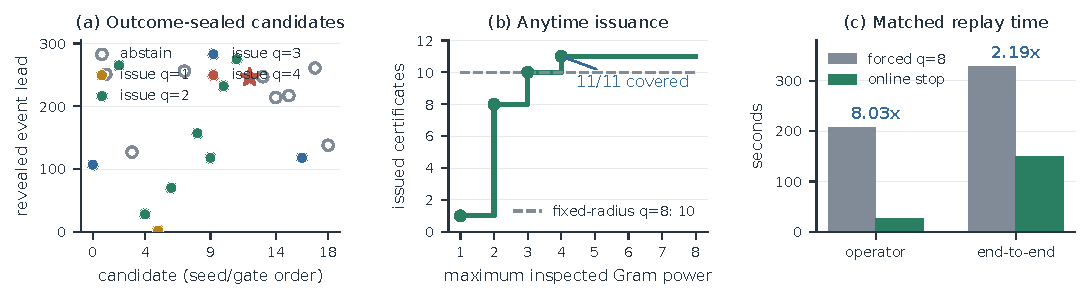
\includegraphics[width=\linewidth]{../figures/paper_transformer_v3_anytime.pdf}
  \caption{Separately sealed response-centered confirmation and executable anytime
  stopping.  (a) All 19 frozen candidates; filled points issue and color gives
  the first valid power.  The red star marks the one v3-only certificate over
  the fixed-radius baseline.  (b) All 11 certificates are available by power
  four; the matched fixed-radius rule issues 10 at power eight.  (c) On one
  sealed candidate, online and forced-q8 executions use identical code and
  streams and return the same bracket, while online stopping cuts operator and
  end-to-end time by $8.03\times$ and $2.19\times$.}
  \label{fig:v3-anytime}
\end{figure}

\subsection{Signed defect propagation controls certificate issuance}

The matched finite-window baseline makes the mechanism unusually sharp.  Of
the 18 frozen Transformer candidates for which the Green operator was queried,
the signed construction issues nine certificates.  The unsigned replacement
$Z_{\rm u}=\kappa\norm{s}$ retains only one.  Eight of nine signed certificates
therefore disappear \emph{solely} because defect direction is discarded.
Across all 18 matched cases, $Z_{\rm u}/Z$ ranges from $83.0$ to $411.5$, with
median $319.7$.  Seventeen cases are ruled out analytically even under the
unsigned method's favorable outer-ball envelope; the sole survivor retains the
same $[30,30]$ event bracket but needs a radius $60.6\times$ larger.
The independently sealed digits study reaches the same conclusion away
from modular arithmetic: signed propagation issues 7/24 cases versus 6/24
unsigned, with the additional 147-step event covered exactly.  Thus the
directional ablation now changes issuance in two datasets and two
parameterizations, including one protocol-primary non-modular case.

On three burned candidates, four development-fixed sweeps reduce median maximum
defect from $8.57\times10^{-3}$ to $5.94\times10^{-8}$ ($1.44\times10^5$) and
make timing errors $(-9,-1,-3)$ exact.  Each costs $H$ HVPs: the path is an
a-posteriori pseudo-orbit solve, not a single-Hessian clock.

\subsection{A directional fourth-order remainder removes one sweep}
\label{sec:block-directional-result}

The cancellation-safe second response contains three known copies of the
parameter correction and one unknown dual direction.  Replacing all four by a
single Euclidean operator norm was the dominant obstruction in a frozen
three-sweep audit.  Corollary~\ref{cor:block-directional-remainder} instead
propagates a polarized block majorant and maximizes only over the free slot.
Across 14 nondevelopment cases, the resulting Taylor-sequence bound is smaller
at every checkpoint; its ratio to the scalar bound ranges from
$9.09\times10^{-5}$ to $1.02\times10^{-3}$, with median
$3.45\times10^{-4}$ ($2{,}899\times$ tighter).

Under the unchanged recorded Green bounds, three holdout closures that
previously abstained now issue $[28,28]$, $[70,70]$, and $[118,118]$; the
development row retains $[2,2]$.  All four brackets exactly match their sealed
four-sweep comparators, and all strict event slacks exceed
$1.36\times10^{-3}$.  Thus an adaptive rule can stop after three predeclared
centerline sweeps on four of 15 records, saving four of 60 centerline sweeps in
the fixed panel without changing its prospective coverage count.

An independent bivariate mixed jet propagates only the coefficient of
$t^3\varepsilon$ rather than materializing the degree-four polynomial.  It
reproduces every checkpoint bound and closure decision with maximum relative
error $4.19\times10^{-15}$.  Its median whole-case runtime improves
$154.31\to115.92$ seconds ($1.33\times$); this misses the prespecified
$2\times$ speed gate because centerline replay dominates, so we claim the
equivalence and sweep saving, not a twofold end-to-end acceleration.  The
audit is post-release, outcome-blind, and makes no new randomized query.

\subsection{Computational scaling with batched operator products}

Post-seal batching accelerates complete replay by $3.00/2.60\times$.  Anytime
stopping exposes all 11 certificates by $q\le4$ (median two) and, in a matched
replay, preserves $[2,2]$ while cutting operator/end-to-end cost by
$8.03\times/2.19\times$.

Post-seal, the cancellation-safe response closes 15/15 Green-evaluable records
versus 11/15, saving 22 powers and 167,250 net objective HVPs; its nine
fourth-order gates retain at least $55.3\times$ headroom.  At $\lambda=4096$,
the amplified secant reproduces $[28,28]$ with $24.4\times$ analytic headroom.
Its 204 outward 192-bit scalar jets bound forcing by $1.31\times10^{-29}$ and
retain $24.41\times$ headroom in 9.80 minutes wall time.  Three rotating-order
triples give 6.56\,s versus 8.10\,s for third-order AD and 26.01\,s for the
next power, a $4.04\times$ paired speedup (Appendix~\ref{app:two-response-audit}).

Corrected-path relinearization removes the mixed coefficient, $0.627\to0$.
In a frozen outcome-blind 15-case panel, every directional bracket survives;
14 stop at four probes and one at eight.  Green applications fall $560\to64$
($8.75\times$) and linearized sweeps $1150\to144$ ($7.99\times$).  Causal
prefix construction is bitwise identical and gives
$9.94/2.09/1.06\times$ speedups at horizons 26/131/299; direct-image release
skips $K^T$ in 4/15 cases.  These post-seal audits leave frozen prospective
counts above unchanged.

Scaled-momentum structure gives a second, orthogonal reduction.  Restricting
the nonlinear gain to $\Pi_\theta K_H\mathcal B$ preserves all 15 brackets,
converts two additional cases to direct-image release, and reduces the matched
staged total from 112 to 96 logical Green sweeps.  A stricter anchor-zero
restriction preserves every bracket but remains at 96 sweeps; it therefore
fails its prespecified promotion gate and is retained as a negative systems
audit rather than advertised as another speedup.

The deterministic neural-jet release sharpens the practical picture further.
Across the complete 15-case operator cohort it preserves eight brackets with
no randomized output-Jacobian query, eliminating 1,432 output operators and
22,912 $q=1$ Gram applications.  All seven unresolved cases retain the
existing probe fallback, so the staged policy still issues 15/15 with identical
brackets.  For the eight deterministic releases the failure upper is the
$10^{-6}$ Green event alone; the minimum strict event-logic slack is
$1.80\times10^{-4}$.  An independent implementation reproduces every
disposition and bracket without reading a future outcome.

The same ingredients were finally composed in one outcome-blind execution on
the sealed seed-366 80\% case ($H=26$).  Three separately launched runs retain
$[2,2]$ in 9.01/11.71/9.21\,s (median 9.21\,s), using four applications of
$K_H$, no application of $K_H^\top$, and no randomized output-Jacobian
operator.  An independent audit reconstructs the analytic closure, event
logic, hashes, and timing ratios from the committed records.  The historical
fixed-$q=8$ cross-batch median was 58.02 minutes, a $378\times$ reduction in
recorded construction time.  On the same seed, anchor, optimizer, and machine,
ordinary continuation takes 0.298\,s for 26 updates and 3.718\,s for 300;
certification is therefore still $30.9\times$ and $2.48\times$ slower,
respectively.  These matched controls separate the practical gain from the
different question of whether revealing the future is cheaper than proving it.

\begin{figure}[t]
  \centering
  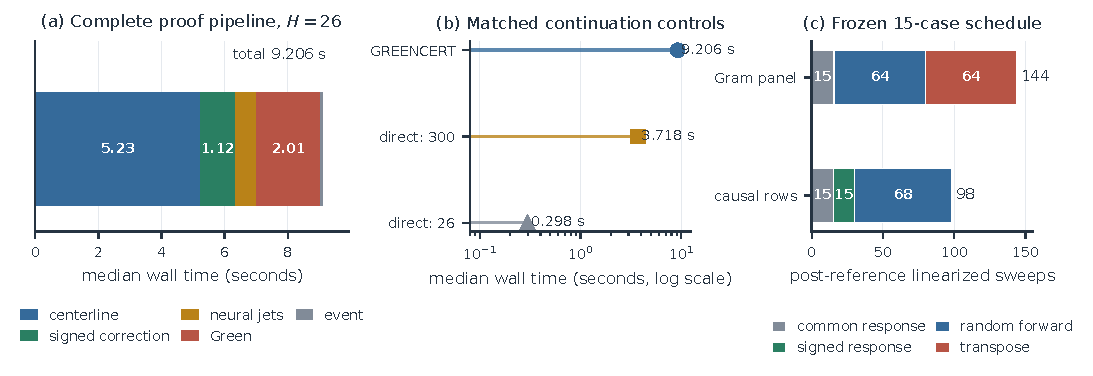
\includegraphics[width=\linewidth]{../figures/paper_composed_runtime.pdf}
  \caption{Measured cost of the fully composed verifier on the sealed
  seed-366, $H=26$ case.  (a) Median phase times over three separately launched
  executions; all retain $[2,2]$.  (b) Same-machine direct-continuation
  controls from the same seed, anchor, and optimizer.  The 58.02-minute
  historical fixed-$q=8$ cross-batch median is excluded from the matched panel.}
  \label{fig:composed-runtime}
\end{figure}

\section{Related Work}

\paragraph{Forecasting and grokking.}
Modular arithmetic is a standard grokking testbed
\citep{power2022grokking,gromov2023modular,mohamadi2024why}; geometry and clocks
predict transitions \citep{notsawo2023predicting,kim2026clock,khanh2026firstpassage},
and local quadratic forecasts reach 150M parameters \citep{meterez2026quadratic}.
\method{} instead certifies finite-window nonlinear validity and first passage.

\paragraph{Trajectory verification and robust training.}
Minute perturbations can send otherwise identical neural-training trajectories
to different solutions \citep{altintas2025butterfly}, making the realized
checkpoint---rather than an interchangeable nearby orbit---the relevant anchor
for an event claim.
Classical shadowing, pseudo-orbit, and radii-polynomial methods certify
trajectory proximity/existence, including in learning dynamics
\citep{chow1989shadowing,chow1992numerical,chow1994global,hammel1987numerical,sauer1991rigorous,lessard2014rigorous,bielecki2004shadowing,orvieto2019shadowing}.
Product-space radii bounds can preserve component structure
\citep{vandenberg2018wright}, while goal-oriented a posteriori methods use
adjoint residuals to control selected quantities of interest
\citep{becker2001optimal}.  Our forcing-subspace result uses the exact
scaled-momentum factorization to close the anchored nonlinear recurrence in
parameter space before transporting it through persistent neural-output
margins.
Robust training/parameter balls \citep{sosnin2026agt,taheri2026barc,weng2020weight},
descent/stability \citep{streeter2022autobound,shi2026ctbab}, and fixed-network
or surrogate verification \citep{wicker2021iterative,mathiesen2026certified,naughton2026certified}
deliver different guarantees.  \method{} propagates signed endogenous defect
on the anchored optimizer orbit to a persistent event bracket.  Matrix-free tools
\citep{pearlmutter1994hvp,kuczynski1992random} and inexact-Newton residual
interfaces \citep{dembo1982inexact} make that causal certificate executable.
The directional fourth-order construction also draws on classical
polarization of symmetric multilinear forms \citep{thomas2014polarization}
and multivariate Taylor-model arithmetic \citep{berz1998taylor}.  Taylor
models have also been integrated with neural-controller reachability
\citep{schilling2022taylor}, while recent neural verification preserves
derivative information inside local reachability bounds
\citep{sharifi2024hessian,entesari2026taylor}.  Here the
polynomial is evaluated on an endogenous optimizer correction and feeds a
finite-window first-passage closure rather than an exogenous input set.

\ifdefined\arxivversion
\begin{table}[t]
\caption{Objects and guarantees delivered by representative approaches.}
\label{tab:novelty}
\centering
\footnotesize
\setlength{\tabcolsep}{3.0pt}
\begin{tabular}{>{\raggedright\arraybackslash}p{0.21\linewidth}>{\raggedright\arraybackslash}p{0.23\linewidth}>{\raggedright\arraybackslash}p{0.24\linewidth}>{\raggedright\arraybackslash}p{0.22\linewidth}}
\toprule
Approach & State/object & Uncertainty or correction & Delivered claim \\
\midrule
Chow--Lin--Palmer;\newline Chow--Palmer
\citep{chow1989shadowing,chow1992numerical}
& numerical pseudo-orbit & right-inverse/Newton correction
& shadowing orbit and proximity bound \\
Lessard--Reinhardt \citep{lessard2014rigorous}
& IVP coefficient sequence & residual and radii polynomial
& rigorous solution enclosure \\
AutoBound/SafeRate \citep{streeter2022autobound}
& one optimizer step & Taylor-remainder majorizer
& certified loss decrease \\
YES training bounds \citep{yeganegi2024yes}
& layerwise data/output mappings & linear/intermediate baselines
& online training-quality and loss bounds \\
Abstract Gradient Training \citep{sosnin2026agt}
& reachable training parameters & training-data perturbation set
& robust prediction after training \\
Barrier robustness \citep{taheri2026barc}
& family of poisoned training trajectories & learned barrier and scenario bound
& terminal poisoning-robustness radius \\
Adaptive SGD stopping \citep{aolaritei2026stopping}
& strongly convex stochastic trajectory & time-uniform confidence sequence
& distance/suboptimality stopping certificate \\
CT-BaB \citep{shi2026ctbab}
& neural controller and input region & verification-aware branch and bound
& post-training Lyapunov stability \\
Certified neural dynamics \citep{wicker2021iterative,mathiesen2026certified}
& learned/Bayesian dynamical model & model or transition uncertainty
& reachability or surrogate-trajectory enclosure \\
Certified Grokking \citep{naughton2026certified}
& fixed published checkpoint and circuit & outward intervals and Lean theorem
& full-domain endpoint and circuit certificate \\
Weight-space robustness \citep{weng2020weight}
& fixed trained network & exogenous parameter ball
& robust prediction at that network \\
\method{}
& optimizer orbit from realized anchor & signed temporal defect and nonlinear tube
& persistent first-passage bracket or abstention \\
\bottomrule
\end{tabular}
\end{table}
\else
\fi

\section{Limitations and broader impact}

The complete certificates currently cover shallow tanh MLPs and a one-block,
13,792-parameter Transformer.  A 102,400-parameter LayerNorm/AdamW audit
transports the required derivatives but does not close the event theorem;
deep networks and stochastic optimization remain open.  At 1.01M parameters,
the matrix-free core takes 11.37 hours before neural-jet construction.  The
fully composed 13,792-parameter $H=26$ verifier now runs in 9.21\,s median,
but matched direct continuation is still $30.9\times$ faster over the needed
window, and this small-model result does not resolve modern-scale closure.  The
events are defined on fixed evaluation sets and coverage is conditional on
issuance, so these are not population guarantees.

The directional-block remainder is presently specialized to the same
normalization-free Transformer and uses analytic block majorants rather than
outward-rounded coefficient arithmetic.  Its post-release audit establishes
theorem tightness and sweep reduction on a frozen panel; it is not counted as
an additional prospective coverage experiment.

The 63 direct 192-bit proofs begin at stored checkpoints.  The 204
amplified-secant jets are outward at 192 bits conditional on stored dyadic
inputs, whereas the upstream Transformer Green products, derivative envelopes,
and output margins remain float64/ideal-PRNG calculations.  The post-seal
$8.75\times$ Green reduction and eight deterministic output releases reuse
frozen analytic envelopes.  They reduce the present cost substantially, but
they do not settle neural-jet construction at modern scale.

\section{Conclusion}

This work asks when a checkpoint-local training clock can support a statement
about the realized future trajectory.  \method{} answers selectively: it
returns a persistent-event bracket when signed response and nonlinear closure
can be verified, and abstains otherwise.  Across the frozen studies, 83/83
issued brackets cover and both inaccurate finite clocks abstain.  The final
implementation preserves all 15 audited Transformer brackets while cutting
Green work $560\to64$; deterministic neural jets remove every output probe in
eight of those cases.  A directional block remainder additionally recovers
three holdout certificates under a three-sweep reference while an independent
mixed jet reproduces every local bound.  Their complete composition turns one sealed Transformer
certificate from an hours-scale historical construction into a reproducible
9.21-second proof object without changing its bracket.

\ifdefined\arxivversion\else\clearpage\fi
\bibliographystyle{plainnat}
\bibliography{references}

\appendix
\raggedbottom

\section{Proofs}
\label{app:proofs}

\begin{proof}[Proof of Theorem~\ref{thm:green}]
Put $e=h-\widetilde z$.  Equation~\eqref{eq:fixedpoint} gives
\begin{equation}
 e=(K_Hs-\widetilde z)+K_HN(\widetilde z+e).
\end{equation}
The anchor terms vanish because $h_0=\widetilde z_0=0$.  For every remaining
transition input, the integral Taylor identity gives
\begin{equation}
 \norm{N_j(\widetilde z_j+e_j)-N_j(\widetilde z_j)}
 \le M\norm{\widetilde z_j}\norm{e_j}
 +\tfrac12M\norm{e_j}^2.
\end{equation}
Since
$\| (\norm{e_j}^2)_j\|_2\le\|e\|_X^2$, we obtain
\begin{equation}
 \|N(\widetilde z+e)-N(\widetilde z)\|_U
 \le Mp\|e\|_X+\tfrac12M\|e\|_X^2.
\end{equation}
The first term in the fixed-point map is bounded by $\alpha$, and
$\|K_HN(\widetilde z)\|_X\le\beta$.  Thus Eq.~\eqref{eq:closure} makes the
continuous exact fixed-point map send the finite-dimensional closed
radius-$E$ sequence ball into itself.  The domain condition validates every
derivative bound.  Brouwer gives a fixed point; causal forward recurrence makes
it unique and equal to the realized trajectory error.
\end{proof}

\begin{proof}[Proof of Corollary~\ref{cor:radius}]
Taylor's theorem yields
\begin{equation}
 \|q\|_U\le\tfrac12M
 \left(\sum_{j=1}^{H-1}\norm{\widetilde z_j}^4\right)^{1/2}
 \le\tfrac12MpZ.
\end{equation}
Hence $\beta=\kappa MpZ/2$ is valid.  Moving the right side of
Eq.~\eqref{eq:closure} to the left gives a convex quadratic in $E$ with
linear coefficient $bp-1$ and constant $Y$.  Conditions
\eqref{eq:response-root} make its discriminant nonnegative and select the
smaller root; the displayed form is obtained by rationalizing the usual
quadratic formula.
\end{proof}

\begin{proof}[Proof of Corollary~\ref{cor:heterogeneous}]
The checkpointwise Taylor bounds give
\begin{align}
 \|N(\widetilde z)\|_U&\le Q,\\
 \|N(\widetilde z+e)-N(\widetilde z)\|_U
 &\le A\|e\|_X+\tfrac12B\|e\|_X^2.
\end{align}
Applying $K_H$ and repeating the self-mapping argument proves
Eq.~\eqref{eq:heterogeneous-closure}.  Finally,
$Q\le MpZ/2$, $A\le Mp$, and $B=M$ show dominance.
\end{proof}

\begin{proof}[Proof of Corollary~\ref{cor:output-recenter}]
Theorem~\ref{thm:green} gives
$\|x_{a+j}-\bar c_j\|\le E$.  Integrating the logit Hessian from $c_j$ to
$\bar c_j$ yields
$\|Df(\bar c_j)\|\le B_{1j}+B_{2j}d_j$.  A second Taylor expansion from
$\bar c_j$ to $x_{a+j}$, followed by the $\sqrt2$ norm of a difference of two
logit coordinates, proves Eq.~\eqref{eq:recentered-marginradius}.  Finally,
$d_j\le p$ and direct subtraction from Eq.~\eqref{eq:marginradius} at
$\varrho=p+E$ leave the nonnegative quantity
$\sqrt2(B_{1j}p+B_{2j}p^2/2)$.
\end{proof}

\begin{proof}[Proof of Proposition~\ref{prop:probe}]
Let $v$ be a unit top eigenvector of $A=T^\top T$.  For each probe,
\begin{equation}
 \lVert A^qg_i\rVert\ge\lVert A\rVert^q|v^\top g_i|.
\end{equation}
The projections are independent standard normals.  By the definition of
$c_\delta$, the probability that all $m$ absolute projections are below
$c_\delta$ is
$(2\Phi(c_\delta)-1)^m=\delta$.  Outside that event,
$\lVert A\rVert^q\le Y_q/c_\delta$ for every $q$ on the same event.  Since
$\lVert A\rVert=\lVert T\rVert^2$, Eq.~\eqref{eq:probe} follows
simultaneously over all inspected powers.
\end{proof}

\begin{proposition}[Residual-corrected inexact Gram powers]
\label{prop:inexact-probe}
Let $A=T^\top T$ and fix an integer $q\ge1$.  Suppose computed iterates
$\widetilde v_{i,0}=g_i$ satisfy
$\max_i\|\widetilde v_{i,\ell+1}-A\widetilde v_{i,\ell}\|\le\xi_\ell$
for $0\le\ell<q$, and put
$\widetilde Y_q=\max_i\|\widetilde v_{i,q}\|$.  Let $R_q$ be the unique
positive root (or zero when all data vanish) of
\begin{equation}
c_\delta R_q^q=\widetilde Y_q+
 \sum_{\ell=0}^{q-1}\xi_\ell R_q^{q-1-\ell}.
\label{eq:inexact-gram}
\end{equation}
Then, on the same probability-$1-\delta$ event as
Proposition~\ref{prop:probe}, simultaneously over inspected powers,
$\|T\|\le\sqrt{R_q}$.  The analogous Frobenius-block statement replaces
$\widetilde Y_q$ and $\xi_\ell$ by block Frobenius norms and $c_\delta$ by the
lower $\delta$-quantile of $\chi_m$.
\end{proposition}

\begin{proof}[Proof of Proposition~\ref{prop:inexact-probe}]
Let $\lambda=\|A\|=\|T\|^2$ and let $v$ be a unit top eigenvector.  On the
single Gaussian event from Proposition~\ref{prop:probe}, some probe $g_i$
satisfies $|v^\top g_i|\ge c_\delta$.  With
$r_{i,\ell}=\widetilde v_{i,\ell+1}-A\widetilde v_{i,\ell}$, telescoping gives
\begin{equation}
A^qg_i=\widetilde v_{i,q}
-\sum_{\ell=0}^{q-1}A^{q-1-\ell}r_{i,\ell}.
\end{equation}
Consequently,
\begin{equation}
c_\delta\lambda^q\le \widetilde Y_q+
\sum_{\ell=0}^{q-1}\xi_\ell\lambda^{q-1-\ell}.
\end{equation}
The polynomial obtained from Eq.~\eqref{eq:inexact-gram} has one positive
leading coefficient and only nonpositive lower coefficients.  Unless every
datum vanishes, Descartes' rule gives exactly one positive root (zero may also
be a root when trailing coefficients vanish).  The displayed inequality thus
forces $\lambda\le R_q$.  The projection event is common to every power.

For the block analogue, collect probes as $G=[g_1\ \cdots\ g_m]$ and use
$c^\chi_{\delta,m}=F^{-1}_{\chi_m}(\delta)$.  Since
$\|v^\top G\|\sim\chi_m$ and
$\|A^qG\|_F\ge\lambda^q\|v^\top G\|$, the same proof applies with
Frobenius terminal and residual norms.  Splitting $\delta$ between the
max-column and chi-block events makes the minimum of their two bounds valid by
a union bound, without another Gram application.
\end{proof}

\begin{corollary}[Precision-adaptive Gram queries]
\label{cor:precision-adaptive}
Fix the operator and Gaussian block in Proposition~\ref{prop:inexact-probe}.
The arithmetic precision, implementation, and residual tolerances at each power
may be selected or refined after inspecting all preceding iterates.  If the
reported $\xi_\ell$ are valid upper bounds relative to the same exact $A$, the
resulting $R_q$ remains a simultaneous probability-$1-\delta$ enclosure for
every inspected power; precision refinement consumes no additional failure
budget.
\end{corollary}

\begin{proof}
On the single top-eigenvector projection event, the telescoping inequality in
the preceding proof is deterministic and holds for every sequence of computed
iterates whose displayed residual bounds are valid.  Adaptive arithmetic
therefore changes only the coefficients of the scalar polynomial, not the
Gaussian event.
\end{proof}

\begin{corollary}[Certificate-aware operator-cap budget]
\label{cor:operator-cap-budget}
Fix $\overline R>0$ and nonnegative $\overline Y,b_0,\ldots,b_{q-1}$ with
\begin{equation}
 \overline Y+\sum_{\ell=0}^{q-1}b_\ell
 \le c_\delta\overline R^q.
\end{equation}
If $\widetilde Y_q\le\overline Y$ and
$\xi_\ell\overline R^{q-1-\ell}\le b_\ell$ for every $0\le\ell<q$, then, on
the same probability-$1-\delta$ event,
$\|T\|\le\sqrt{\overline R}$.  Each failed local check may be recomputed at
higher precision without another probe draw.
\end{corollary}

\begin{proof}
The assumptions make $\overline R$ a supersolution of
Eq.~\eqref{eq:inexact-gram}.  Proposition~\ref{prop:inexact-probe} and
Corollary~\ref{cor:precision-adaptive} complete the claim.
\end{proof}

Inexact Krylov and variable-accuracy eigensolver theory likewise study
perturbed matrix--vector products
\citep{simoncini2003inexact,simoncini2005variable}; recent residual-based
Chebyshev iteration demonstrates the mixed-precision opportunity at large
scale \citep{kodali2025residual}.  Proposition~\ref{prop:inexact-probe}
specializes residual transport to the one-sided randomized norm enclosure
required here.

\begin{proof}[Proof of Proposition~\ref{prop:predictable}]
Let $E_n$ be the single-block event from Proposition~\ref{prop:probe} for
operator $T_n$.  Conditional independence gives
$\Pr(E_n^c\mid\mathcal F_{n-1})\le\delta_n$.  Therefore
\begin{equation}
 \Pr\!\left(\bigcup_{n\ge1}E_n^c\right)
 \le\sum_{n\ge1}\mathbb E\!\left[
 \Pr(E_n^c\mid\mathcal F_{n-1})\right]
 \le\mathbb E\sum_{n\ge1}\delta_n\le\delta.
\end{equation}
Every power and stopping decision for query $n$ is already valid on $E_n$.
\end{proof}

\begin{proof}[Quadratic defect contraction, Eq.~\eqref{eq:defectcontraction}]
After one sweep, the new path defect is exactly
\begin{equation}
 r^{(k+1)}_j=G(c^{(k)}_j+z^{(k)}_j)-G(c^{(k)}_j)
 -DG(c^{(k)}_j)z^{(k)}_j.
\end{equation}
The integral Taylor bound gives
$\norm{r^{(k+1)}_j}\le M\norm{z^{(k)}_j}^2/2$.  Taking maxima and using
$\max_j\norm{z^{(k)}_j}\le
\kappa_{\infty,H}\max_i\norm{r^{(k)}_i}$ proves the claim.
\end{proof}

\begin{proposition}[Inexact variational-sweep residual]
\label{prop:inexact-sweep}
For a reference path $c$, let
$r_j=G(c_j)-c_{j+1}$ and $J_j=DG(c_j)$.  Let
$\widetilde r_j$ be a computed defect and let an anchor-fixed correction
$\widetilde z_0=0$ have recurrence residual
\begin{equation}
 d_j=\widetilde z_{j+1}-J_j\widetilde z_j-\widetilde r_j.
\end{equation}
The defect $r'_j$ of the recentered path $c'=c+\widetilde z$ satisfies the
exact identity
\begin{equation}
 \boxed{r'_j=N_j(\widetilde z_j)+(r_j-\widetilde r_j)-d_j.}
 \label{eq:inexact-sweep}
\end{equation}
Consequently, if $DG$ is $M_j$-Lipschitz on the connecting segment,
$\|r_j-\widetilde r_j\|\le\sigma_j$, and $\|d_j\|\le\tau_j$, then
\begin{equation}
 \|r'_j\|\le\tfrac12M_j\|\widetilde z_j\|^2+\sigma_j+\tau_j.
 \label{eq:inexact-sweep-bound}
\end{equation}
\end{proposition}

\begin{proof}
Substitute the definition of $r_j$ and add and subtract
$J_j\widetilde z_j$:
\begin{align}
r'_j
&=G(c_j+\widetilde z_j)-c_{j+1}-\widetilde z_{j+1}\\
&=N_j(\widetilde z_j)+r_j+J_j\widetilde z_j-\widetilde z_{j+1},
\end{align}
which is Eq.~\eqref{eq:inexact-sweep}.  Taylor's integral remainder and the
triangle inequality give Eq.~\eqref{eq:inexact-sweep-bound}.
\end{proof}

The residual term parallels classical inexact Newton forcing conditions
\citep{dembo1982inexact}; here it is resolved checkpointwise on the
anchor-fixed causal sequence and carried into a first-passage verifier.

\begin{corollary}[Residualized two-response interface]
\label{cor:two-response-residual}
Let $\widehat\kappa\ge\|K_H\|$.  Suppose $\widetilde s$ and an anchor-fixed
$\widetilde z$ obey
\begin{equation}
 \|s-\widetilde s\|_U\le\sigma_s,\qquad
 \|d^z\|_U\le\tau_z,\qquad
 d^z_j=\widetilde z_{j+1}-J_j\widetilde z_j-\widetilde s_j.
\end{equation}
Set $q_j=N_j(\widetilde z_j)$.  If a computed $\widetilde q$ and anchor-fixed
$\widetilde y$ obey
\begin{equation}
 \|q-\widetilde q\|_U\le\sigma_q,\qquad
 \|d^q\|_U\le\tau_q,\qquad
 d^q_j=\widetilde y_{j+1}-J_j\widetilde y_j-\widetilde q_j,
\end{equation}
then Theorem~\ref{thm:green} is valid with
\begin{equation}
 \alpha=\widehat\kappa(\sigma_s+\tau_z),\qquad
 \beta=\|\widetilde y\|_X+\widehat\kappa(\sigma_q+\tau_q).
 \label{eq:two-response-residual}
\end{equation}
In particular, Proposition~\ref{prop:inexact-probe} may supply
$\widehat\kappa$ from residual-certified low-precision Gram products.
\end{corollary}

\begin{proof}
The recurrence definitions give the exact identities
$\widetilde z=K_H(\widetilde s+d^z)$ and
$\widetilde y=K_H(\widetilde q+d^q)$.  Hence
\begin{align}
 \|K_Hs-\widetilde z\|_X
 &\le\widehat\kappa(\sigma_s+\tau_z),\\
 \|K_Hq\|_X
 &\le\|\widetilde y\|_X+\widehat\kappa(\sigma_q+\tau_q).
\end{align}
These are precisely the $\alpha$ and $\beta$ hypotheses of
Theorem~\ref{thm:green}.
\end{proof}

\begin{corollary}[Cancellation-safe directional second response]
\label{cor:directional-two-response}
In the setting of Corollary~\ref{cor:two-response-residual}, suppose $G_j$ is
$C^3$ on $c_j+t\widetilde z_j$, $0\le t\le1$, and
\begin{equation}
 \sup_{0\le t\le1}\|D^3G_j(c_j+t\widetilde z_j)\|\le L_j.
\end{equation}
Define
\begin{equation}
 q^{(2)}_j=\tfrac12D^2G_j(c_j)
 [\widetilde z_j,\widetilde z_j],\qquad
 \sigma_2=
 \left(\sum_{j=0}^{H-1}
 \left(\tfrac16L_j\|\widetilde z_j\|^3\right)^2\right)^{1/2}.
 \label{eq:directional-q2}
\end{equation}
If $\|\widetilde q^{(2)}-q^{(2)}\|_U\le\sigma_{\rm ar}$ and an
anchor-fixed $\widetilde y$ has recurrence residual
\begin{equation}
 d^y_j=\widetilde y_{j+1}-J_j\widetilde y_j-
 \widetilde q^{(2)}_j,\qquad \|d^y\|_U\le\tau_y,
\end{equation}
then Theorem~\ref{thm:green} may use
\begin{equation}
 \boxed{\beta=\|\widetilde y\|_X+
 \widehat\kappa(\sigma_2+\sigma_{\rm ar}+\tau_y).}
 \label{eq:directional-two-response}
\end{equation}
For scaled momentum
$G(\theta,w)=(\theta-r,r)$,
$r=\mu w+\eta\nabla F(\theta)$, and
$\widetilde z_j=(a_j,b_j)$,
\begin{equation}
 q^{(2)}_j=\frac{\eta}{2}
 \left(-D^3F(\theta_j)[a_j,a_j,\cdot],
        D^3F(\theta_j)[a_j,a_j,\cdot]\right).
 \label{eq:momentum-q2}
\end{equation}
Consequently, $\|D^4F\|\le L_{F,4,j}$ on the parameter segment permits
$L_j=\sqrt2\,\eta L_{F,4,j}$.
\end{corollary}

\begin{proof}
Third-order Taylor expansion gives
$q_j=q^{(2)}_j+r^{(3)}_j$ with
$\|r^{(3)}_j\|\le L_j\|\widetilde z_j\|^3/6$, hence
$\|q-q^{(2)}\|_U\le\sigma_2$.  The recurrence identity
$\widetilde y=K_H(\widetilde q^{(2)}+d^y)$ then yields
\begin{equation}
 \|K_Hq\|_X\le\|\widetilde y\|_X+
 \widehat\kappa(\sigma_2+\sigma_{\rm ar}+\tau_y).
\end{equation}
For scaled momentum, only the gradient term is nonlinear; differentiating it
twice and three times gives Eqs.~\eqref{eq:momentum-q2} and the stated
fourth-objective bound.
\end{proof}

\begin{corollary}[Directional block remainder]
\label{cor:block-directional-remainder}
In Corollary~\ref{cor:directional-two-response}, decompose parameter space as
the orthogonal sum $\Theta=\bigoplus_{b=1}^B\Theta_b$, with projections
$\pi_b$.  For checkpoint $j$, let $a_j$ be the parameter component of
$\widetilde z_j$ and $r_{j,b}=\|\pi_ba_j\|_2$.  Suppose that on
$\theta_j+ta_j$, $0\le t\le1$, the symmetric fourth derivative of $F$ admits
a nonnegative symmetric four-linear polarized block majorant
$\mathcal P_{j,4}$:
\begin{equation}
 |D^4F(\theta_j+ta_j)[h_1,h_2,h_3,h_4]|
 \le \mathcal P_{j,4}(s(h_1),s(h_2),s(h_3),s(h_4)),
 \quad s(h)_b=\|\pi_bh\|_2.
 \label{eq:polarized-block-majorant}
\end{equation}
This symmetry entails no loss: average any valid nonnegative four-linear
majorant over all $4!$ slot permutations.  Symmetry of $D^4F$ preserves the
inequality, and diagonal evaluation is unchanged.
Write $P_{j,4}(s)=\mathcal P_{j,4}(s,s,s,s)$.  Then the scalar Taylor term in
Eq.~\eqref{eq:directional-q2} may be replaced by
\begin{equation}
 \sigma_{\rm blk}=
 \left\{\sum_{j=0}^{H-1}
 \left(\frac{\sqrt2\,\eta}{24}
 \|\nabla P_{j,4}(r_j)\|_2\right)^2\right\}^{1/2}.
 \label{eq:block-directional-sigma}
\end{equation}
Consequently Eq.~\eqref{eq:directional-two-response} remains valid with
$\sigma_2$ replaced by $\sigma_{\rm blk}$.
\end{corollary}

\begin{proof}
For a unit dual direction $u$, put $t_b=\|\pi_bu\|_2$; orthogonality gives
$\|t\|_2=1$.  Symmetry and homogeneity imply
\begin{equation}
 \mathcal P_{j,4}(r_j,r_j,r_j,t)
 =\tfrac14\nabla P_{j,4}(r_j)^\top t
 \le\tfrac14\|\nabla P_{j,4}(r_j)\|_2.
\end{equation}
Taylor's integral remainder for the objective gradient contributes another
factor $1/6$.  The scaled-momentum map places the same parameter remainder in
two state blocks with opposite signs, contributing $\sqrt2\eta$.  Taking the
Euclidean sequence norm gives Eq.~\eqref{eq:block-directional-sigma}.
\end{proof}

The implementation obtains $P_{j,4}$ coefficientwise through nonnegative
sum, product, affine-map, and smooth-composition rules.  A linear-cost
alternative propagates only $D_t^k$ and $D_t^kD_\varepsilon$ for $k\le3$;
the terminal $D_t^3D_\varepsilon$ coefficient is exactly the vector
$\nabla P_{j,4}(r_j)/4$ and avoids materializing degree-four monomials.

\begin{corollary}[Amplified-secant second response]
\label{cor:amplified-secant}
In the setting of Corollary~\ref{cor:two-response-residual}, choose
$\lambda_j>0$ and suppose $G_j$ is $C^3$ on
$c_j+t\widetilde z_j$ for
$0\le t\le\max\{1,\lambda_j\}$, with
$\|D^3G_j\|\le L_j$ there.  Define
\begin{equation}
 q_j^{[\lambda_j]}=
 \frac{G_j(c_j+\lambda_j\widetilde z_j)-G_j(c_j)
       -\lambda_jJ_j\widetilde z_j}{\lambda_j^2},
 \quad
 \sigma_{\rm sec}=
 \left(\sum_{j=0}^{H-1}
 \left[\frac{|\lambda_j-1|}{6}L_j
 \|\widetilde z_j\|^3\right]^2\right)^{1/2}.
 \label{eq:amplified-secant}
\end{equation}
If $\|\widetilde q^{[\lambda]}-q^{[\lambda]}\|_U\le\sigma_{\rm ar}$
and an anchor-fixed $\widetilde y$ has recurrence residual at most $\tau_y$,
then Theorem~\ref{thm:green} may use
\begin{equation}
 \boxed{\beta=\|\widetilde y\|_X+
 \widehat\kappa(\sigma_{\rm sec}+\sigma_{\rm ar}+\tau_y).}
 \label{eq:amplified-secant-response}
\end{equation}
If the unscaled secant numerator has arithmetic error at most $\varepsilon_j$,
checkpoint $j$ contributes at most
$A_j|\lambda_j-1|+\varepsilon_j/\lambda_j^2$, where
$A_j=L_j\|\widetilde z_j\|^3/6$.  For a $\lambda$-independent
$\varepsilon_j$ and $A_j,\varepsilon_j>0$, the unconstrained optimum over
$\lambda_j\ge1$ is
\begin{equation}
 \lambda_j^\star=
 \max\left\{1,(2\varepsilon_j/A_j)^{1/3}\right\},
 \label{eq:optimal-amplification}
\end{equation}
clipped by the derivative domain and error budget.
If $\varepsilon_j=0$, take $\lambda_j=1$; if $A_j=0$, take the largest
admissible amplification.
\end{corollary}

\begin{proof}
Taylor's integral identity gives
\begin{equation}
 \frac{N_j(t\widetilde z_j)}{t^2}
 =\int_0^1(1-s)D^2G_j(c_j+st\widetilde z_j)
 [\widetilde z_j,\widetilde z_j],ds.
\end{equation}
Subtracting the identities at $t=1$ and $t=\lambda_j$, then integrating the
$D^3G_j$ drift, gives
$\|N_j(\widetilde z_j)-q_j^{[\lambda_j]}\|
\le|\lambda_j-1|L_j\|\widetilde z_j\|^3/6$.
Equation~\eqref{eq:amplified-secant-response} follows from the residualized
two-response identity.  Finally, differentiating
$A_j(\lambda_j-1)+\varepsilon_j/\lambda_j^2$ gives
Eq.~\eqref{eq:optimal-amplification}.
\end{proof}

\begin{corollary}[Fresh-probe forcing and Green-image residual]
\label{cor:residual-probe}
Let $e\in\R^D$ be fixed before fresh independent
$g_i\sim\mathcal N(0,I_D)$, $1\le i\le m$.  Suppose outward scalar intervals
$[\ell_i,u_i]$ contain $g_i^\top e$, and define
\begin{equation}
 B=\max_i\max\{|\ell_i|,|u_i|\},\qquad
 c_\delta=\Phi^{-1}\!\left(\frac{1+\delta^{1/m}}2\right).
 \label{eq:residual-probe}
\end{equation}
Then, with conditional probability at least $1-\delta$,
\begin{equation}
 \boxed{\|e\|_2\le B/c_\delta.}
 \label{eq:residual-probe-bound}
\end{equation}
More sharply, for fixed $K:U\to X$, fresh $h_i\sim\mathcal N(0,I_X)$, and
outward intervals containing
$\langle K^\top h_i,e\rangle_U=\langle h_i,Ke\rangle_X$, the same construction
gives $\|Ke\|_X\le B/c_\delta$.  Hence, with
$e_{\rm ar}=q^{[\lambda]}-\widetilde q^{[\lambda]}-d^y$, one may use
\begin{equation}
 \beta=\|\widetilde y\|_X+\widehat\kappa\sigma_{\rm sec}
       +B/c_\delta,
 \label{eq:green-image-residual}
\end{equation}
without multiplying numerical error by $\widehat\kappa$.  Alternatively,
probing $q^{[\lambda]}$ itself gives the response-free interface
$\beta=\widehat\kappa(\sigma_{\rm sec}+B/c_\delta)$.

For scaled momentum, let a forcing probe at checkpoint $j$ be
$g_j=(g_{\theta,j},g_{w,j})$ and put $w_j=g_{w,j}-g_{\theta,j}$.  Its
checkpoint contribution is the scalar bivariate jet
\begin{equation}
 g_j^\top q_j^{[\lambda]}=\frac{\eta}{\lambda^2}
 \left[D_{w_j}F(\theta_j+\lambda a_j)-D_{w_j}F(\theta_j)
 -\lambda D^2_{w_j,a_j}F(\theta_j)\right].
 \label{eq:scalar-secant-projection}
\end{equation}
and a sequence projection sums these contributions.  Green-image probing uses
$g=K^\top h$.  All adaptive choices must precede the fresh, prebudgeted block;
computed adjoints require outward recurrence-error accounting.
\end{corollary}

\begin{proof}
Conditional on nonzero fixed $e$, the variables $g_i^\top e/\|e\|$ are iid
standard normal.  The probability that every absolute projection is below
$c_\delta$ is $(2\Phi(c_\delta)-1)^m=\delta$; outward intervals only increase
their maximum.  Apply the same argument to $Ke$ and use adjointness for the
Green-image claim.  Since
$Kq-\widetilde y=K(q-q^{[\lambda]})+Ke_{\rm ar}$,
Eq.~\eqref{eq:green-image-residual} follows.  The response-free inequality is
the triangle bound $\|Kq\|_X\le\widehat\kappa
(\sigma_{\rm sec}+\|q^{[\lambda]}\|_U)$.  The momentum identity follows by
splitting the state probe and writing gradient inner products as directional
derivatives.
\end{proof}

\begin{corollary}[Corrected-path relinearized Green closure]
\label{cor:relinearized-green}
Let $v_0=0$, $b_j=c_j+v_j$, and
\begin{equation}
 r^v_j=v_{j+1}-J_jv_j-s_j,\qquad
 \bar s_j=G(b_j)-b_{j+1},\qquad \bar J_j=DG(b_j).
 \label{eq:corrected-defect}
\end{equation}
Let $\bar K_H$ be the anchor-fixed causal Green operator generated by
$\bar J_0,\ldots,\bar J_{H-1}$.  Assume the pairwise local envelope
\begin{equation}
 \|DG(c_j+u)-DG(c_j+w)\|\le M\|u-w\|
 \label{eq:pairwise-drift}
\end{equation}
whenever $\|u\|,\|w\|\le\rho$.  Suppose
$\bar\kappa\ge\|\bar K_H\|$ and $Y$ is a valid bound, including numerical
error, on $\|\bar K_H\bar s\|_X$.  If
\begin{equation}
 \bar D=1-2\bar\kappa MY\ge0,\qquad
 E=\frac{2Y}{1+\sqrt{\bar D}},\qquad
 \max_{0\le j<H}\|v_j\|+E\le\rho,
 \label{eq:corrected-closure}
\end{equation}
then
\begin{equation}
 \|x_{a+1:a+H}-b_{1:H}\|_X\le E.
 \label{eq:corrected-tube}
\end{equation}
Moreover, the corrected defect obeys the exact cancellation-safe identity
\begin{equation}
 \boxed{\bar s_j=N_j(v_j)-r^v_j.}
 \label{eq:corrected-defect-identity}
\end{equation}
Thus an exact variational response ($r^v=0$) leaves second-order forcing, and
the closure $Y+\bar\kappa ME^2/2\le E$ contains no mixed term.  Any verified
response, fresh-probe, or Green-image bound from
Corollary~\ref{cor:residual-probe} may supply $Y$.
\end{corollary}

\begin{proof}
Expanding $G(c_j+v_j)$ around $c_j$ proves
Eq.~\eqref{eq:corrected-defect-identity}.  For
$e_j=x_{a+j}-b_j$, causal recurrence gives
\begin{equation}
 e=\bar K_H\bar s+\bar K_H\bar N(e),\qquad
 \bar N_j(e_j)=G(b_j+e_j)-G(b_j)-\bar J_je_j.
\end{equation}
Equation~\eqref{eq:pairwise-drift} and the domain condition imply
$\|\bar N(e)\|_U\le M\|e\|_X^2/2$.  Hence
$Y+\bar\kappa ME^2/2\le E$ makes the exact finite-dimensional map self-mapping.
Brouwer gives a fixed point, causal forward recurrence makes it unique, and the
stable smaller quadratic root is Eq.~\eqref{eq:corrected-closure}.
\end{proof}

\begin{corollary}[Scaled-momentum parameter-forcing closure]
\label{cor:parameter-forcing}
In Corollary~\ref{cor:relinearized-green}, let
\begin{equation}
 G(\theta,w)=(\theta-r,r),\qquad
 r=\mu w+\eta\nabla F(\theta),
 \label{eq:scaled-momentum-factorization}
\end{equation}
and let $\Pi_\theta(\delta\theta,\delta w)=\delta\theta$.  Define the
checkpointwise injection
\begin{equation}
 \mathcal Bq_j=(-\eta q_j,\eta q_j)
\end{equation}
and the anchor shift
\begin{equation}
 \mathcal S(p_1,\ldots,p_H)=(0,p_1,\ldots,p_{H-1}).
 \label{eq:anchor-shift}
\end{equation}
Let $Q_0$ prepend a zero block to an $(H-1)$-block forcing sequence and put
\begin{equation}
 T_{\theta,0}=\Pi_\theta\bar K_H\mathcal BQ_0.
 \label{eq:parameter-green}
\end{equation}
Suppose, on the declared parameter domains,
\begin{equation}
 R_j(u)=\nabla F(\theta_j+u)-\nabla F(\theta_j)-H_ju,
 \qquad \|R_j(u)\|\le \tfrac12L\|u\|^2.
 \label{eq:objective-gradient-remainder}
\end{equation}
If
\begin{equation}
 \kappa_\theta\ge\|T_{\theta,0}\|,\qquad
 Y_\theta\ge\|\Pi_\theta\bar K_H\bar s\|_X,
\end{equation}
and
\begin{equation}
 D_\theta=1-2\kappa_\theta L Y_\theta\ge0,\qquad
 E_\theta=\frac{2Y_\theta}{1+\sqrt{D_\theta}},
 \label{eq:parameter-root}
\end{equation}
with every pointwise parameter ball of radius $E_\theta$ inside its declared
domain, then
\begin{equation}
 \left(\sum_{j=1}^{H}
 \|\Pi_\theta(x_{a+j}-b_j)\|^2\right)^{1/2}\le E_\theta.
 \label{eq:parameter-tube}
\end{equation}
For exact operator quantities,
\begin{equation}
 \|T_{\theta,0}\|L
 \le \sqrt2\,\eta\|\bar K_H\|L,\qquad
 \|\Pi_\theta\bar K_H\bar s\|_X
 \le\|\bar K_H\bar s\|_X.
 \label{eq:parameter-dominance}
\end{equation}
Thus the parameter closure is never worse than the full-state corrected
closure for a parameter-defined event.  Replacing $L$ by checkpointwise
$L_j$ and querying
$\Pi_\theta\bar K_H\mathcal B
\operatorname{diag}(L_j)Q_0$ gives an equally valid, weakly sharper
curvature-profiled coefficient.
\end{corollary}

\begin{proof}
For $e_j=x_{a+j}-b_j$, write
$p=(\Pi_\theta e_1,\ldots,\Pi_\theta e_H)$.  Equation
\eqref{eq:scaled-momentum-factorization} gives the exact remainder
factorization
\begin{equation}
 G(b_j+e_j)-G(b_j)-\bar J_je_j
 =\mathcal B R_j(\Pi_\theta e_j),
\end{equation}
with $R_j$ from Eq.~\eqref{eq:objective-gradient-remainder}.  Because
$e_0=0$, the first remainder block is zero.  Causal substitution therefore
yields the closed parameter equation
\begin{equation}
 p=\Pi_\theta\bar K_H\bar s+
 T_{\theta,0}R_+(\mathcal Sp).
 \label{eq:parameter-fixedpoint}
\end{equation}
For $\|p\|_X\le E$,
\begin{equation}
 \|R_+(\mathcal Sp)\|_U
 \le \frac L2
 \left(\sum_{j=1}^{H-1}\|p_j\|^4\right)^{1/2}
 \le \frac L2\|p\|_X^2.
\end{equation}
Hence the right side of Eq.~\eqref{eq:parameter-fixedpoint} maps the
radius-$E_\theta$ parameter ball into itself.  Brouwer gives a fixed point;
lifting it through $\bar K_H$ solves the full causal recurrence, whose forward
trajectory from the realized anchor is unique.  Equation
\eqref{eq:parameter-root} is the cancellation-safe smaller root.  Finally,
$\|\Pi_\theta\|=\|Q_0\|=1$ and
$\|\mathcal B\|=\sqrt2\eta$, proving
Eq.~\eqref{eq:parameter-dominance}.  The checkpointwise statement follows by
absorbing $\operatorname{diag}(L_j)$ into the input side of the same operator.
\end{proof}

\begin{corollary}[Deterministic neural-jet release]
\label{cor:analytic-jet-release}
In Corollary~\ref{cor:relinearized-green}, suppose the optimizer objective is
mean cross entropy composed with a neural logit map $f_j$, plus quadratic
weight decay, and the scaled-momentum learning rate is $\eta$.  On each outer
ball $B(c_j,\rho)$ let
\begin{equation}
 \|Df_j\|\le A_j,\qquad \|D^2f_j\|\le B_j,
 \qquad \|D^3f_j\|\le C_j.
 \label{eq:analytic-jet-envelope}
\end{equation}
Then Eq.~\eqref{eq:pairwise-drift} holds with
\begin{equation}
 M_{\rm jet}=\max_{1\le j<H}\sqrt2\eta
 \left(2A_j^3+\tfrac32A_jB_j+\sqrt2C_j\right).
 \label{eq:analytic-jet-M}
\end{equation}
If the corrected closure issues with this $M_{\rm jet}$ and
$p=\max_j\|v_j\|$, every true-class-versus-competitor margin satisfies
\begin{equation}
 |m_{iq}(x_{a+j})-m_{iq}(c_j)|
 \le \sqrt2 A_j(p+E).
 \label{eq:analytic-jet-margin}
\end{equation}
Strict event logic based on Eq.~\eqref{eq:analytic-jet-margin} therefore needs
no randomized output-Jacobian operator.  A policy may try this deterministic
release first and instantiate the sharper output probe only after failure;
such predictable fallback adds no probability charge to cases released by the
deterministic screen and preserves the preallocated family bound otherwise.
\end{corollary}

\begin{proof}
For cross entropy,
$\|D\ell\|\le\sqrt2$, $\|D^2\ell\|\le1/2$, and
$\|D^3\ell\|\le2$.  The third-order chain rule gives
\begin{equation}
 \|D^3(\ell\circ f_j)\|
 \le2A_j^3+3(1/2)A_jB_j+\sqrt2C_j.
\end{equation}
Averaging examples cannot increase the norm, and quadratic weight decay has
zero third derivative.  The scaled-momentum Jacobian changes by at most
$\sqrt2\eta$ times the objective-Hessian change, proving
Eq.~\eqref{eq:analytic-jet-M}.  The corrected tube lies in the declared outer
ball because $p+E\le\rho$.  The mean-value theorem bounds each logit change by
$A_j(p+E)$; subtracting two logits gives Eq.~\eqref{eq:analytic-jet-margin}.
Proposition~\ref{prop:predictable} supplies the fallback accounting.
\end{proof}

\begin{corollary}[Nested-prefix direct-image/Gram release]
\label{cor:direct-image-prefix}
Let $T$ be fixed before iid $g_i\sim\mathcal N(0,I)$ are drawn, and fix
$1\le m_1<\cdots<m_L$, integers $q_\ell\ge1$, and
$\delta_\ell>0$ with $\sum_\ell\delta_\ell\le\delta$.  Put
\begin{equation}
 c_\ell=\Phi^{-1}\!\left(
 \frac{1+\delta_\ell^{1/m_\ell}}{2}\right).
\end{equation}
Then with probability at least $1-\delta$, simultaneously for every prefix,
\begin{equation}
 \|T\|\le\frac{\max_{i\le m_\ell}\|Tg_i\|}{c_\ell},
 \qquad
 \|T\|\le
 \left(\frac{\max_{i\le m_\ell}\|(T^TT)^{q_\ell}g_i\|}{c_\ell}
 \right)^{1/(2q_\ell)}.
 \label{eq:direct-gram-release}
\end{equation}
Hence one may inspect the direct release, apply $T^T$ to the cached images only
if needed, and stop at the first issuing prefix.  For a predeclared operator
family, summing $\delta_{n,\ell}$ over operators and prefixes gives the
family-wise bound.
\end{corollary}

\begin{proof}
For a unit top right singular vector $v$ and $Tv=\|T\|u$,
$\|Tg_i\|\ge\|T\||v^Tg_i|$ and
$\|(T^TT)^qg_i\|\ge\|T\|^{2q}|v^Tg_i|$.  Prefix $\ell$ fails only if all
$m_\ell$ absolute standard-normal projections are below $c_\ell$, an event of
probability $\delta_\ell$.  A union bound proves simultaneous validity; direct
screening, Gram fallback, and stopping are functions of already valid bounds.
\end{proof}

\begin{proposition}[Causal prefix commutation]
\label{prop:causal-prefix}
Let $A_H(x_0)$ be the horizon-$H$ affine reference and $R_H$ one anchor-fixed
variational recentering sweep.  If $P_h$ retains states $0{:}h$ and neither
construction truncates before $h\le H$, then
\begin{equation}
 P_hA_H(x_0)=A_h(x_0),\qquad
 P_hR_H(c)=R_h(P_hc),\qquad
 P_hR_H^SA_H(x_0)=R_h^SA_h(x_0).
 \label{eq:prefix-commutation}
\end{equation}
All $S$ sweeps may therefore be pipelined in one forward pass with
$O(Hd+Sd)$ rather than $O(SHd)$ path storage, and construction may stop when a
sealed horizon or first persistent predicted event is reached.
\end{proposition}

\begin{proof}
The affine state at $j+1$ uses only its state at $j$.  In one recentering
sweep, $d_{j+1}=DG(c_j)d_j+G(c_j)-c_{j+1}$ depends only on
$(c_j,c_{j+1},d_j)$.  Induction in time proves both prefix identities; induction
over the sweep index proves the last.  Pipelining retains the preceding sweep's
current/next states and each sweep's current correction, while storing only the
final path.
\end{proof}

\begin{proposition}[Persistent first-passage bracket]
If $n^-_j\le n_j\le n^+_j$ for $0\le j\le H$ and the finite endpoints
$L,U\in\{0,\ldots,H-K+1\}$ are defined by
Eq.~\eqref{eq:persistentbracket}, then $T_{r,K}$ is finite and
$L\le T_{r,K}\le U$.
\end{proposition}

\begin{proof}
Before $L$, every length-$K$ block contains an offset with $n^+<r$, so the
true block cannot be entirely above gate.  At $U$, every offset has
$n^-\ge r$, so the true block is above gate throughout.
\end{proof}

\begin{proposition}[Witness-sparse, predictable, role-fused event transport]
\label{prop:witness-sparse}
Let $P_j$ certify that the gate holds at $j$, and $F_j$ certify that it fails.
A bracket $[L,U]$ is valid if $P_j$ holds for
$j=U,\ldots,U+K-1$ and a set $W^-$ of certified failure times intersects
every interval $[t,t+K-1]$ for $t<L$.  For a fixed set of available failure
times, greedily selecting the rightmost available point in the earliest-ending
uncovered interval gives a minimum-cardinality $W^-$.  If the optimizer depends
on training outputs $f_{\rm tr}$ and the event on evaluation outputs
$f_{\rm ev}$, it is sufficient to bound derivatives of $f_{\rm tr}$ at
transition-input states and derivatives of $f_{\rm ev}$ only at the success
and failure-witness times.  Witness times may be acquired predictably from
centerline margins and prior certificate results using fresh prebudgeted probe
blocks.  At a time requiring both roles, one bound on
$D(f_{\rm tr}\oplus f_{\rm ev})$ may replace the two component queries.
\end{proposition}

\begin{proof}
The success window proves $T_{r,K}\le U$, while a certified failure in every
earlier length-$K$ interval proves $T_{r,K}\ge L$.  For interval stabbing,
replace the first point of any optimal solution that hits the earliest-ending
uncovered interval by that interval's rightmost available point; this cannot
uncover a later-ending interval.  Induction proves greedy optimality.  Finally,
optimizer drift factors only through the objective and $f_{\rm tr}$, whereas
event margins factor only through $f_{\rm ev}$ at the logical witnesses.
Predictable acquisition is covered by Proposition~\ref{prop:predictable}.
Finally, each component Jacobian is an output projection of the direct-sum
Jacobian, so its norm is no larger.  Intersecting the prebudgeted operator
events completes the claim.
\end{proof}

\paragraph{Affine launch-cost consequence.}
Let $Q\subseteq\{1,\ldots,H\}$ be the $q$ event-query times, and let one call
on $n$ examples cost $a+bn$.  Dense, separate-role, and fused costs are
respectively
\begin{align*}
C_{\rm d}&=Ha+bHn_{\rm all},\\
C_{\rm s}&=(H-1+q)a+b\{(H-1)n_{\rm tr}+qn_{\rm ev}\},\\
C_{\rm f}&=(H-1+\mathbf1_{\{H\in Q\}})a
 +b\{(H-1)n_{\rm tr}+qn_{\rm ev}\}.
\end{align*}
Thus fusion removes exactly
$(q-\mathbf1_{\{H\in Q\}})a$ from the separate path.  Separate roles beat
the dense baseline only if
$b[Hn_{\rm all}-(H-1)n_{\rm tr}-qn_{\rm ev}]>(q-1)a$.
This explains the observed launch-overhead regression without asserting a
hardware-independent runtime guarantee.

\begin{lemma}[Scaled-momentum derivative drift]
If $\lVert\nabla^2F(\theta+u)-\nabla^2F(\theta)\rVert\le L\norm{u}$, then the
map in Eq.~\eqref{eq:momentum} satisfies
$\lVert DG(x+h)-DG(x)\rVert\le\sqrt2\eta L\norm{h}$.
\end{lemma}

\begin{proof}
Only the parameter-to-update Hessian block changes.  Applied to
$(d\theta,dw)$, the Jacobian difference is
$(-\eta\Delta H d\theta,\eta\Delta H d\theta)$, whose norm is at most
$\sqrt2\eta L\norm{h}\norm{(d\theta,dw)}$.
\end{proof}

\section{Complete analytic Transformer derivative envelope}
\label{app:transformer-jet}

This section derives the deterministic first-, second-, and third-order neural
envelopes used in every Transformer certificate.  Random-direction tests are
useful regression checks, but they are not part of the validity argument.  The
argument below follows the computational graph line by line.

\subsection{Norms, parameter blocks, and diagonal jets}

Every activation tensor is flattened and given its Euclidean (equivalently,
Frobenius) norm.  Matrix parameters use the Frobenius norm as coordinates and
the spectral norm when acting on an activation.  The complete parameter vector
is partitioned into 14 orthogonal blocks:
\begin{center}
\small
\begin{tabular}{rll}
\toprule
$b$ & block & contents \\
\midrule
0 & embedding & token and position embeddings jointly \\
1--3 & attention weights & $W_Q,W_K,W_V$ (disjoint row slices) \\
4--6 & attention biases & $b_Q,b_K,b_V$ (disjoint slices) \\
7--8 & attention output & $W_O,b_O$ \\
9--10 & feed-forward 1 & $W_1,b_1$ \\
11--12 & feed-forward 2 & $W_2,b_2$ \\
13 & readout & $W_R$ \\
\bottomrule
\end{tabular}
\end{center}
The grouped/sliced blocks are still orthogonal: the squared block Frobenius
norms sum to the squared norm of the original flat perturbation.  Hence a unit
direction $u$ has block radii $s_b=\norm{u_b}$ satisfying
$\sum_b s_b^2=1$.

For a smooth tensor-valued stage $f$, write $P_k^f(s)$ for a polynomial with
nonnegative coefficients such that
\begin{equation}
 \norm{D^k f(\theta)[u,\ldots,u]}\le P_k^f(s),\qquad k=1,2,3.
 \label{eq:jet-diagonal}
\end{equation}
The restriction to a repeated direction loses nothing for the Euclidean
multilinear norm.  Indeed, each scalarization of $D^k f$ is a symmetric
$k$-linear form on a real Hilbert space; Banach's theorem gives equality
between its multilinear norm and the norm of its diagonal homogeneous
polynomial.  Dualizing the output gives the same result for tensor-valued $f$
\citep{carando2019symmetric}.  Thus a valid bound on
Eq.~\eqref{eq:jet-diagonal}, maximized over $\sum_b s_b^2\le1$, bounds the full
Fr\'echet derivative norm.

For a monomial $m(s)=\prod_b s_b^{\alpha_b}$ of degree
$d=\sum_b\alpha_b$, Lagrange multipliers give the exact sphere maximum
\begin{equation}
 \sup_{\sum_b s_b^2\le1}m(s)
 =\prod_{b:\alpha_b>0}\left(\frac{\alpha_b}{d}\right)^{\alpha_b/2}.
 \label{eq:monomial-sphere}
\end{equation}
We maximize a nonnegative polynomial by summing these exact monomial maxima.
This can be conservative for a sum, but it is always valid and never exceeds
the older scalar rule that sets every $s_b=1$.

\subsection{Primitive jet rules}

Represent a stage by $\mathcal J(f)=(V_f,P_1^f,P_2^f,P_3^f)$, where
$V_f\ge\norm{f}$ on the relevant input set.  All inequalities below follow
from the triangle inequality, submultiplicativity of Frobenius/spectral norms,
and the ordinary Fr\'echet product and chain rules.

For addition, $h=f+g$,
\begin{equation}
 V_h=V_f+V_g,\qquad P_k^h=P_k^f+P_k^g.
 \label{eq:jet-add}
\end{equation}
For a bilinear contraction $h=\alpha f g$ (matrix multiplication included),
\begin{align}
V_h&=|\alpha|V_fV_g,\nonumber\\
P_1^h&=|\alpha|(P_1^fV_g+V_fP_1^g),\nonumber\\
P_2^h&=|\alpha|(P_2^fV_g+2P_1^fP_1^g+V_fP_2^g),\nonumber\\
P_3^h&=|\alpha|(P_3^fV_g+3P_2^fP_1^g
 +3P_1^fP_2^g+V_fP_3^g).
 \label{eq:jet-product}
\end{align}
For an elementwise or rowwise smooth map $h=\phi\circ f$ with
$\norm{D^k\phi}\le a_k$ on the stage range,
\begin{align}
P_1^h&=a_1P_1^f,\nonumber\\
P_2^h&=a_1P_2^f+a_2(P_1^f)^2,\nonumber\\
P_3^h&=a_1P_3^f+3a_2P_1^fP_2^f+a_3(P_1^f)^3.
 \label{eq:jet-smooth}
\end{align}
Products of the $P_k$ in Eqs.~\eqref{eq:jet-product}--\eqref{eq:jet-smooth}
are polynomial convolutions over block labels, so mixed derivatives and their
combinatorial multiplicities are retained exactly before the sphere relaxation.

For a parameterized affine stage with sequence length $\ell$,
\begin{equation}
 h(X,W,b)=XW^\top+\mathbf 1_\ell b^\top,
 \label{eq:affine-stage}
\end{equation}
we assign the weight jet $(\lVert W\rVert_{\rm op},s_W,0,0)$ and bias jet
$(\sqrt\ell\norm{b},\sqrt\ell s_b,0,0)$ and apply
Eq.~\eqref{eq:jet-product} plus Eq.~\eqref{eq:jet-add}.  This is valid because
\begin{equation}
 \lVert XW^\top\rVert_F\le\lVert X\rVert_F\lVert W\rVert_{\rm op},\qquad
 \lVert\mathbf 1_\ell b^\top\rVert_F=\sqrt\ell\norm{b}.
 \label{eq:affine-norms}
\end{equation}
On a radius-$R$ parameter ball we replace $\lVert W\rVert_{\rm op}$ by
$\lVert W_0\rVert_{\rm op}+R$ and $\norm{b}$ by $\norm{b_0}+R$; using the full
radius for each value bound is conservative even though the derivative
polynomial retains the sharper block allocation.

\subsection{Global activation constants}

The Gaussian-error linear unit is
$\operatorname{GELU}(x)=x\Phi(x)$, with standard-normal density $\varphi$.
Direct differentiation gives
\begin{align}
g'(x)&=\Phi(x)+x\varphi(x),\nonumber\\
g''(x)&=(2-x^2)\varphi(x),\nonumber\\
g'''(x)&=(x^3-4x)\varphi(x).
\end{align}
Elementary one-dimensional maximization yields
\begin{equation}
 \sup|g'|<1.13,\qquad \sup|g''|<0.80,\qquad \sup|g'''|<2.
 \label{eq:gelu-constants}
\end{equation}
For an elementwise map these scalar constants also bound the induced
Euclidean multilinear derivatives, since
$\norm{x_1\odot\cdots\odot x_k}\le\prod_i\norm{x_i}$.

For $p=\operatorname{softmax}(x)$, let
$C(p)=\operatorname{diag}(p)-pp^\top$.  The categorical covariance bound gives
$\lVert C(p)\rVert_{\rm op}\le1/2$.  If $q=C(p)h$, then
\begin{equation}
 DC(p)[h]=\operatorname{diag}(q)-qp^\top-pq^\top,
\end{equation}
whose norm is at most $3\norm{h}/2<2\norm{h}$.  Differentiating once more and
using $\norm{p}\le1$, $\norm{q}\le\norm{h}/2$, and
$\norm{DC(p)[k]}\le3\norm{k}/2$ gives the conservative bound $5<6$ for the
third derivative.  Therefore the implementation uses
\begin{equation}
 (a_1,a_2,a_3)_{\rm softmax}=(1/2,2,6).
 \label{eq:softmax-constants}
\end{equation}
The causal mask is a constant translation before softmax and contributes no
derivative.  Rowwise application is block diagonal, so the same constants hold
under the flattened Frobenius norm.

\subsection{One-block causal Transformer graph}

The certified architecture has sequence length three, one normalization-free
causal attention block, one GELU feed-forward block, residual additions, and a
linear readout.  For each of the finite $p^2$ input pairs the implementation
applies the following graph.

\paragraph{Embedding.}
Token lookup and positional addition are linear.  A sequence may repeat an
input token, and all three positions vary.  The joint lookup operator is
bounded by $\sqrt3$, so
\begin{equation}
 \mathcal J(X_0)=(V_{X_0},\sqrt3,s_{\rm emb},0,0).
\end{equation}

\paragraph{Queries, keys, and values.}
For $A\in\{Q,K,V\}$,
\begin{equation}
 A=X_0W_A^\top+\mathbf1_3b_A^\top.
\end{equation}
The three weight slices and three bias slices are disjoint blocks.  Each jet is
given by Eqs.~\eqref{eq:jet-product} and \eqref{eq:affine-norms}.

\paragraph{Scores and attention.}
Reshaping into heads is an isometry.  With head dimension $d_h$,
\begin{equation}
 S=QK^\top/\sqrt{d_h},\qquad P=\operatorname{softmax}_{\rm row}(S+\mathcal M),
 \qquad A=PV.
\end{equation}
The score and attended-value jets use Eq.~\eqref{eq:jet-product}; the
probability jet uses Eqs.~\eqref{eq:jet-smooth} and
\eqref{eq:softmax-constants}.  Matrix contraction is safe because
$\lVert QK^\top\rVert_F\le\lVert Q\rVert_F\lVert K\rVert_F$ and
$\lVert PV\rVert_F\le\lVert P\rVert_F\lVert V\rVert_F$.

\paragraph{Output projection, residuals, feed-forward, and readout.}
The remaining graph is
\begin{align}
X_1&=X_0+(AW_O^\top+\mathbf1_3b_O^\top),\nonumber\\
U&=X_1W_1^\top+\mathbf1_3b_1^\top,\qquad V=g(U),\nonumber\\
X_2&=X_1+(VW_2^\top+\mathbf1_3b_2^\top),\nonumber\\
f_\theta(x)&=(X_2)_{3,:}W_R^\top.
\end{align}
Affine stages use Eq.~\eqref{eq:affine-stage}, residuals use
Eq.~\eqref{eq:jet-add}, and GELU uses Eqs.~\eqref{eq:jet-smooth} and
\eqref{eq:gelu-constants}.  Selecting the last token is nonexpansive.  This
completes the line-by-line derivation of the three output derivative
polynomials.  For hash-preserving reproducibility, the sealed implementation
upper-bounds the bias-free readout by the larger affine family that also permits
an auxiliary bias perturbation.  This is a model-class relaxation, not a stated
graph component: algebraically it adds one nonnegative degree-one monomial and
changes no higher derivative polynomial.  Deleting that monomial gives the
exact bias-free graph and weakly decreases every downstream bound, so all
sealed certificates remain valid.  A released regression test checks this
identity in both scalar and block-polynomial implementations.

\subsection{Making center values valid on the complete ball}

The input set is finite, so every center-stage maximum $V_i^0$ is evaluated
exactly over all $p^2$ pairs in the real-arithmetic specification.  Center
values alone are not ball-valid.  Let $B_{1,i}(V^0+\Delta,R)$ be the first
derivative polynomial for stage $i$ after substituting proposed inflated stage
values.  All its coefficients are nonnegative and it is coordinatewise
nondecreasing.  We seek a post-fixed inflation
\begin{equation}
 \Delta_i\ge R B_{1,i}(V^0+\Delta,R)\quad\text{for every stage }i.
 \label{eq:value-postfixed}
\end{equation}

\begin{lemma}[Ball-valid value chain]
\label{lem:value-chain}
If Eq.~\eqref{eq:value-postfixed} holds, then every stage value on
$B(\theta_0,R)$ is bounded by $V_i^0+\Delta_i$, and the derivative polynomials
computed with those values enclose $D^k f$ for $k=1,2,3$ throughout the ball.
\end{lemma}

\begin{proof}
Proceed in computational-graph order.  For any $\theta_0+h$ with
$\norm{h}\le R$, the integral mean-value identity and the inductively valid
upstream stage values give
\begin{equation}
 \norm{f_i(\theta_0+h)}
 \le V_i^0+R B_{1,i}(V^0+\Delta,R)\le V_i^0+\Delta_i.
\end{equation}
The primitive rules above then apply with valid values at every stage.  Their
composition encloses all derivatives through order three.
\end{proof}

The implementation starts at $\Delta=0$ and repeatedly replaces each
coordinate by the maximum of its current value and the right side of
Eq.~\eqref{eq:value-postfixed}.  This is monotone iteration.  The frozen
Transformer records use a relative $10^{-9}$ binary64 consistency tolerance,
so this check is part of their disclosed numerical rather than exact-real
layer.  A post-seal strict wrapper instead inflates each iterate with directed
binary64 \texttt{nextafter} steps until every displayed inequality is
literally satisfied.  On the shortest sealed issuance, recomputation finds 338
frozen stage inequalities with positive but tiny deficits (maximum
$1.90\times10^{-23}$ absolute and $5.15\times10^{-14}$ relative); the strict
wrapper removes all of them, leaves the rounded derivative jets unchanged, and
reproduces the issued bracket.  This hardens the internal post-fixed check but
is not a substitute for outward real arithmetic.  The same positivity gives a
useful monotonicity fact.

\begin{lemma}[Radius monotonicity]
\label{lem:jet-monotone}
For $0\le R_1\le R_2$, the analytic post-fixed envelopes may be chosen so that
$B_k(R_1)\le B_k(R_2)$ for $k=1,2,3$.
\end{lemma}

\begin{proof}
Every primitive coefficient, value inflation, and weight/bias enlargement is
nonnegative and nondecreasing in $R$.  A post-fixed point for $R_2$ is therefore
also an upper solution for the $R_1$ inequalities.  Substitution into the
nonnegative derivative polynomials proves the claim.
\end{proof}

Lemma~\ref{lem:jet-monotone} is what makes the strong unsigned baseline audit
decisive: once its required radius contains the signed ball, failure even with
the smaller-ball $M$ rules out closure under the same analytic envelope.

\subsection{Cross-entropy and optimizer-map drift}

For one example, cross-entropy is
$\ell_y(z)=-z_y+\log\sum_q e^{z_q}$.  With $p=\operatorname{softmax}(z)$,
\begin{equation}
 \norm{D\ell_y}=\norm{p-e_y}\le\sqrt2,qquad
 \norm{D^2\ell_y}=\norm{C(p)}\le\tfrac12.
\end{equation}
The same calculation used above gives the generous global bound
$\norm{D^3\ell_y}\le2$.  If $B_1,B_2,B_3$ enclose the first three derivatives
of the per-example logit map on the parameter ball, the third-order chain rule
therefore gives
\begin{equation}
 \norm{D^3(\ell_y\circ f_\theta)}
 \le 2B_1^3+\tfrac32B_1B_2+\sqrt2 B_3.
 \label{eq:ce-third-bound}
\end{equation}
An average over examples obeys the same maximum bound.  Weight decay is
quadratic and contributes no Hessian drift.  The center logit Jacobian is
bounded separately by the matrix-free Gram probe; if its bound is
$\widehat B_{1,0}$, then
\begin{equation}
 B_1(R)=\widehat B_{1,0}+B_2(R)R
\end{equation}
is ball-valid.  Substitution into Eq.~\eqref{eq:ce-third-bound} yields the
objective Hessian-Lipschitz constant $L$.

In scaled momentum coordinates $x=(\theta,w=\eta v)$,
\begin{equation}
G(\theta,w)=(\theta-r,r),\qquad
r=\mu w+\eta\nabla F(\theta).
\end{equation}
Only the Hessian block changes with the state.  Consequently
\begin{equation}
 \norm{DG(x+h)-DG(x)}\le\sqrt2\eta L\norm{h},
\end{equation}
which is the implemented $M=\sqrt2\eta L$.  The anchor error is exactly zero,
so only transitions leaving $c_1,\ldots,c_{H-1}$ enter the maximum.

\subsection{Output-margin transport}

The parameter component of a scaled-state perturbation has norm at most the
full state perturbation.  Taylor's theorem gives, for each logit vector,
\begin{equation}
 \norm{f(\theta+h)-f(\theta)}
 \le B_1R+\tfrac12B_2R^2.
\end{equation}
A true-versus-competitor margin is the inner product with $e_y-e_q$, whose
norm is $\sqrt2$.  Thus every margin changes by at most
\begin{equation}
 E=\sqrt2\left(B_1R+\tfrac12B_2R^2\right).
\end{equation}
Strictly positive lower margins certify correct examples.  A strictly negative
upper margin certifies an incorrect example.  Counting these statements gives
the lower/upper accuracy paths used by the persistent first-passage corollary.

\section{Randomness and finite-precision claim boundary}
\label{app:randomness-numerics}

\subsection{What the Gaussian theorem randomizes}

Proposition~\ref{prop:probe} is an exact-arithmetic statement about independent
$N(0,I)$ vectors.  Its probability is over probe randomness only---not over
training seeds, examples, candidate selection, or future outcomes.  The frozen
protocol declares the complete operator family before training, divides the
$10^{-6}$ family budget over that maximum family, and makes no randomized query
during screening.

The executable uses an OS-random master nonce frozen before training.  Each
complete operator identity is domain-separated by SHA-256 into a 63-bit seed;
a registry rejects unknown identities, repeated queries, and seed collisions.
PyTorch then maps that seed deterministically to pseudorandom normal variates.
Domain separation prevents accidental stream reuse, but deterministic PRNG
outputs are not literally independent mathematical Gaussians.  Accordingly,
the Transformer statement is a family-wise high-confidence numerical claim
under the standard ideal-PRNG model.  It is not an unconditional theorem about
the fixed bit strings produced by a particular generator.  A deterministic
replacement would require an independently certified spectral-norm enclosure.

\subsection{Robust theorem for computational error}

The abstract Green theorem already admits explicit computational remainder.
If $\widetilde s$ approximates the defect and a computed response
$\widetilde z_0=0$ has exact-real recurrence residual
\begin{equation}
 d_j=\widetilde z_{j+1}-J_j\widetilde z_j-\widetilde s_j,
\end{equation}
then
\begin{equation}
 \lVert s-\widetilde s\rVert_U\le\sigma,\quad
 \lVert d\rVert_U\le\tau
 \quad\Longrightarrow\quad
 \lVert K_Hs-\widetilde z\rVert_X\le\kappa(\sigma+\tau).
\end{equation}
Using $\alpha=\kappa(\sigma+\tau)$ in Theorem~\ref{thm:green} is sufficient.  Likewise,
outward upper bounds on $\kappa,M,B_1,B_2$ and outward lower bounds on strict
margin slacks preserve the event certificate.

The Transformer implementation evaluates the neural jets, HVP/VJP products,
Gram iterates, and margins in deterministic float64 and does not yet supply
nonzero verified $\sigma,\tau$ for every operation.  Its 9/9 and 11/11 results
therefore remain high-confidence numerical certificates rather than
computer-assisted exact-real proofs.  The fixed-radius cohort has minimum
closure slack $0.1445$ and minimum strict output slack
$2.67\times10^{-5}$.  In contrast, the WDBC and digits tanh
confirmations enclose all 63 issued events with direct 192-bit outward
continuations whose recurrences are independent of the randomized Green event;
the dense modular study provides an additional outward-verified regime.  These
direct passes validate the retained exact-real event brackets, not every Green
inequality.  This distinction is stated in the abstract, results table, and
limitations.


\section{Complete frozen protocols}
\label{app:protocols}

\paragraph{WDBC.}
The Wisconsin Diagnostic Breast Cancer data contain 569 labeled examples with
30 real-valued features \citep{wolberg1995wdbc,street1993nuclear}.  Fresh seeds
101--124 use class-stratified 341/113/115 train/trigger/certification splits and
train-only standardization.  A width-8 tanh MLP (266 parameters) runs 1,000
full-batch float64 GD updates with $\eta=0.005$ and weight decay 0.001.  At
90/92.5/95\% gates with $K=10$, the selector freezes the first five-update
checkpoint with train accuracy at least 80\% and trigger accuracy in
$[\tau-10\%,\tau)$.  Its API cannot materialize certification rows; candidates
and certificates are sealed before future trajectories are joined.  The method
fixes $H=300$, four sweeps, $m=8,q=4$, a $10^{-6}$ family budget, and the
smallest closure root.  Inspected development seeds 0--7 fixed every choice
before the method seal.  The separate 192-bit verifier begins at zero radius on
each exact dyadic anchor and propagates a direct one-step tube without a Green
norm or randomized probe.

\paragraph{Digits.}
The scikit-learn digits data contain 1,797 normalized $8\times8$ images from
the UCI Optical Recognition test set \citep{alpaydin1998digits}.  The protocol
freezes digit parity, seeds 501--512, parity-stratified 1,077/359/361 splits,
train-only standardization, and a width-8 tanh MLP (538 parameters) trained by
600 full-batch GD updates with $\eta=0.03$.  The 90/92.5\% gates use $K=10$,
the WDBC anchor rule, $H=400$, three sweeps, $m=8,q=4$, and a $10^{-6}$
family budget.  Inspected development seeds 0--2 fix the sweep budget; signed
and unsigned methods receive the same centerline.  Code, fresh seeds, and the
primary signed-only endpoint are sealed before training, under the WDBC
selection/outcome barrier.  The post-outcome 192-bit verifier directly encloses
the exact-real optimizer map without a Green norm or probe.

\paragraph{Fixed-radius Transformer cohort.}
Fresh seeds 331--354 train one-block causal Transformers on addition modulo 17:
model dimension 32, four heads, GELU width 128, residuals, no normalization or
dropout, and 13,792 parameters.  The 27,584-dimensional momentum state runs
6,000 full-batch float64 updates with $\eta=0.01$, $\mu=0.9$, and weight decay
0.01; each seed splits 289 examples into 173/58/58.  The protocol fixes
70/80/90\% gates, $K=25$, $H=300$, and four sweeps.  A 40-update causal scan
freezes the first predicted event after train accuracy reaches 99\%, trigger
accuracy reaches $\max(50\%,\tau-20\%)$, and the current certification count
lies one to three examples below gate.  It fixes $R=2Z$, $m=16,q=8$, and a
$10^{-6}$ budget over 21,744 possible operators.  Future trajectories remain
inaccessible through certificate sealing.  This selector reads the current
certification count, although the certification set is disjoint from trigger;
hence the cohort is prospective and outcome-sealed, not untouched by selection.

\paragraph{Response-centered Transformer cohort.}
Fresh seeds 355--378 repeat the model, optimizer, splits, gates, and outcome
barrier.  Before these runs, code and constants are sealed for four variational
sweeps, outer domain $\rho=2Z$, the response-centered root in
Corollary~\ref{cor:radius}, and a shared-probe ladder $q=1,\ldots,8$.  The first
power whose nonlinear closure and persistent-event margins both pass issues.  A
response-aware lower bound $\kappa\ge\max(1,Z/\|s\|_X)$ permits zero-query
abstention; the matched baseline reuses the power-8 quantities with radius
$2Z$.  The family budget is $10^{-6}$ over the worst-case 24-by-3 candidate
universe.  One selector/constructor horizon mismatch among 19 sealed candidates
is retained as an outcome-blind construction abstention under the pre-outcome
execution amendment in Appendix~\ref{app:v3-audit}.

\paragraph{Diagnostic and numerical studies.}
Three earlier Transformer candidates (seeds 321--322) with already known
outcomes supply the excluded 0--4-sweep audit.  The post-seal unsigned audit
replaces $Z=\norm{K_Hs}$ by $Z_{\rm u}=\kappa\norm{s}$ while preserving the
right inverse, outer-ball envelope, and smallest closure root; it is a matched
scalar Euclidean comparator, not a claim about componentwise or Taylor-model
validators.  Other post-seal diagnostics batch the same 16 committed probes and
test exact products for a two-block LayerNorm/AdamW map.  Dense mod-11 MLPs
(827 parameters) provide 192-bit outward evaluation of every issued inequality,
and a disjoint mod-13 study (1,933 parameters) supplies HVP-only
active/complement uncertainty.  Direct 192-bit continuations independently
retain every issued WDBC and digits bracket.

\section{Complete WDBC confirmation and outward audit}
\label{app:wdbc}

\begin{figure}[H]
  \centering
  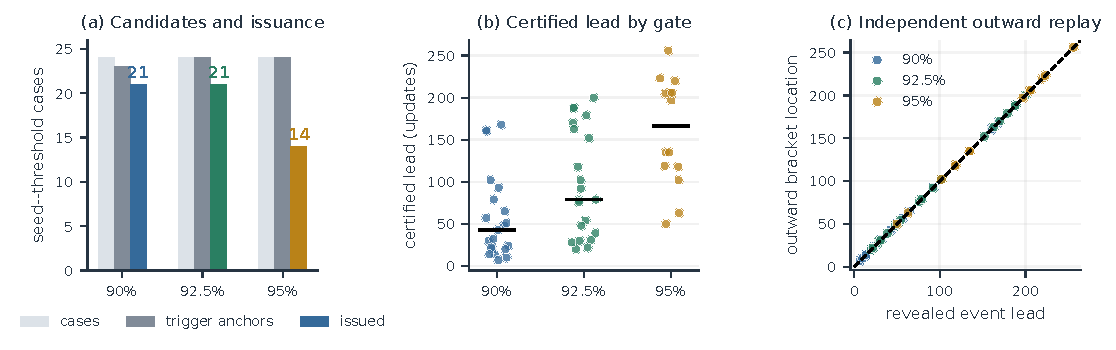
\includegraphics[width=\linewidth]{../figures/paper_real_data_confirmation.pdf}
  \caption{Fully frozen WDBC confirmation.  (a) Candidate and issuance counts
  remain high as the gate rises.  (b) Higher transitions are certified farther
  in advance.  (c) All 56 outward-retained singleton brackets equal the
  subsequently revealed crossing; jitter only separates coincident points.}
  \label{fig:wdbc}
\end{figure}

The downloaded WDBC CSV has SHA-256 prefix
\texttt{FF5FC1F247213DB}.
The frozen method, candidate manifest, certificate manifest, and final
independent audit have SHA-256 prefixes
\texttt{3408AF37C0395926}, \texttt{F552930042296C89},
\texttt{0444FE25E4C414B9}, and \texttt{54DA92445CC7E909},
respectively; full hashes are in the artifact manifest.  The source seal covers
16 protocol and implementation files.  The independent
auditor verifies the complete hash chain, reconstructs every checkpoint
exactly, recomputes candidate and issuance dispositions, and evaluates every
persistent bracket without importing the experiment's aggregation helper.

The 72-case candidate disposition is 71 frozen trigger-only anchors and one
case with no anchor.  The certificate disposition is 56 issued and 15
abstentions because the frozen centerline has no future event on the newly
opened certification split.  The 56 issued cases query 56 Green operators; the
original Green route has realized ideal-Gaussian union bound
$7.78\times10^{-7}$.  Minimum float64
closure and output slacks are 0.9999999907 and
$2.3753122\times10^{-5}$, respectively.  The realized sequence error differs
from the radius by at most $1.27\times10^{-14}$ in absolute terms; the outward
pass resolves this binary64 diagnostic rather than treating a strict
floating-point comparison as proof.

The 192-bit verifier is a separately hashed direct validated-continuation
program.  It treats every stored
binary64 datum as an exact dyadic input and outward-encloses tanh network
evaluation, exact-Hessian construction, eigenpair residuals, optimizer
Jacobians, one-step defect recurrences, nonlinear drift, and event margins.
Its anchor radius is zero and its recurrence contains no Green norm, probe, or
PRNG call; therefore the Gaussian event above is not a condition of an
outward-retained bracket.
Across 40 unique seed-anchor tubes it verifies 5,089 state transitions.  The
largest optimizer-Jacobian norm is 1.00744, the largest Hessian-evaluation
enclosure error is $3.74\times10^{-12}$, and the largest eigen-numerical error
is $5.87\times10^{-11}$.  All 56 singleton brackets remain identical and all
56 cover.

\begin{table}[H]
\caption{WDBC confirmation by prespecified gate.  Coverage is conditional on
issuance; each issued bracket is a singleton.}
\label{tab:wdbc}
\centering
\small
\setlength{\tabcolsep}{7pt}
\begin{tabular}{rrrrrr}
\toprule
Gate & Candidates & Issued & Covered & Median lead & Max lead \\
\midrule
90\%   & 23/24 & 21 & 21/21 & 43  & 168 \\
92.5\% & 24/24 & 21 & 21/21 & 79  & 200 \\
95\%   & 24/24 & 14 & 14/14 & 166 & 256 \\
\midrule
All     & 71/72 & 56 & 56/56 & 79  & 256 \\
\bottomrule
\end{tabular}
\end{table}

\begin{table}[H]
\caption{Post-seal matched WDBC validated-numerics comparison on the 56
Green-issued coordinates.  Direct timing excludes construction of the shared
four-sweep centerline, biasing the runtime ratio in its favor.}
\label{tab:wdbc-direct}
\centering
\small
\setlength{\tabcolsep}{5pt}
\begin{tabular}{lrrrr}
\toprule
Validator & Events & Covered & Random condition & Aggregate time \\
\midrule
\method{} event records & 56 & 56/56 & Gaussian Green bound & 33.88 min \\
Direct 192-bit continuation & 56 & 56/56 & none & 7.12 h \\
\bottomrule
\end{tabular}
\end{table}

The direct/GreenCert aggregate ratio is $12.61\times$.  The direct comparator
was not run on the 15 Green abstentions, so Table~\ref{tab:wdbc-direct} compares
matched rigor and cost rather than unconditional availability.  Both methods
use the same four-sweep reference; only the direct one-step tube dispenses with
the Green closure.  Exact-real scope begins at the stored checkpoint and does
not retroactively verify the PyTorch/BLAS training execution.

\section{Complete prospective digits audit}
\label{app:digits-audit}

The bundled scikit-learn digits arrays have SHA-256
\texttt{F6D9E39F37DC45D3}.  The method, candidate, and pre-outcome certificate
seals have prefixes \texttt{9901CD1A0E3FEABF},
\texttt{BFA31D77050F164D}, and \texttt{99AC9C628AFB4FC9}.
The method seal predates every seed 501--512 artifact; the candidate seal
predates the first full-split loader call; and the certificate seal records
seven signed, six unsigned, and one signed-only issuance before any future
certification trajectory exists.  Reconstruction after the seal has zero
checkpoint error.

All 24 seed--gate cases become candidates.  Twelve reach a Green query and
consume a realized ideal-Gaussian family budget of $5\times10^{-7}$.  Seven
signed certificates issue across six seeds and all seven cover.  Table
\ref{tab:digits-issued} records the complete issued set; the supplement records
all 17 abstentions.  The primary signed-only event has ample separation:
$0.2369<1$ signed versus $13.018>1$ unsigned, with strict output slack
$1.43\times10^{-5}$.

A post-seal verifier independently rebuilds each three-sweep path and propagates
a zero-radius 192-bit Arb tube under the exact-real full-batch map.  It imports
neither the Green radius nor its Gaussian probe.  All seven distinct
seed--anchor tubes reach their horizons; all seven outward brackets are
identical to Table~\ref{tab:digits-issued} and cover.  Maximum radius is
$5.07\times10^{-9}$, minimum strict logic slack is $1.46\times10^{-5}$,
maximum Hessian interval-row radius is $2.18\times10^{-11}$, and maximum
eigensolver numerical error is $1.39\times10^{-10}$.  This includes the
signed-only $[147,147]$ event.

\begin{table}[H]
\caption{All issued certificates in the prospective non-modular digits study.
Lead is relative to the frozen anchor; every bracket contains the
revealed event.  U marks whether the matched unsigned method also issues.}
\label{tab:digits-issued}
\centering
\small
\setlength{\tabcolsep}{4.5pt}
\begin{tabular}{rrrrrrrr}
\toprule
Seed & Gate & Anchor & Lead & Bracket & Signed stat. & Unsigned stat. & U \\
\midrule
503 & 90\%   & 35 & 49  & [49,49]   & $4.9{\times}10^{-6}$ & $9.0{\times}10^{-5}$ & yes \\
504 & 90\%   & 60 & 49  & [49,49]   & $1.9{\times}10^{-8}$ & $5.0{\times}10^{-7}$ & yes \\
506 & 90\%   & 20 & 70  & [70,70]   & $2.1{\times}10^{-5}$ & $4.4{\times}10^{-4}$ & yes \\
507 & 90\%   & 35 & 117 & [117,117] & 0.0137 & 0.2944 & yes \\
509 & 90\%   & 35 & 147 & [147,147] & 0.2369 & 13.018 & no \\
512 & 90\%   & 20 & 42  & [42,42]   & $3.5{\times}10^{-8}$ & $7.8{\times}10^{-7}$ & yes \\
512 & 92.5\% & 35 & 73  & [73,73]   & $2.8{\times}10^{-4}$ & 0.0086 & yes \\
\bottomrule
\end{tabular}
\end{table}

The post-seal selectivity audit also compares every finite frozen prediction
with its revealed event.  Table~\ref{tab:digits-inaccurate} gives the only two
inaccurate finite centerlines.  Both were rejected by deterministic early
closure before an outcome or randomized probe was available.

\begin{table}[H]
\caption{Every inaccurate finite forecast in the prospective digits study.
Error is prediction minus event; the lower bound is the favorable
$\kappa\ge1$ closure statistic, so a value above one proves abstention without
querying the Green norm.}
\label{tab:digits-inaccurate}
\centering
\small
\setlength{\tabcolsep}{5pt}
\begin{tabular}{rrrrrrrl}
\toprule
Seed & Gate & Anchor & Prediction & Event & Error & Lower bound & Disposition \\
\midrule
510 & 92.5\% & 45 & 218 & 219 & $-1$ & 6,512 & early abstain \\
511 & 90\%   & 50 & 358 & 361 & $-3$ & 4,505 & early abstain \\
\bottomrule
\end{tabular}
\end{table}

\section{Complete fresh Transformer audit}
\label{app:transformer-audit}

\begin{figure}[H]
  \centering
  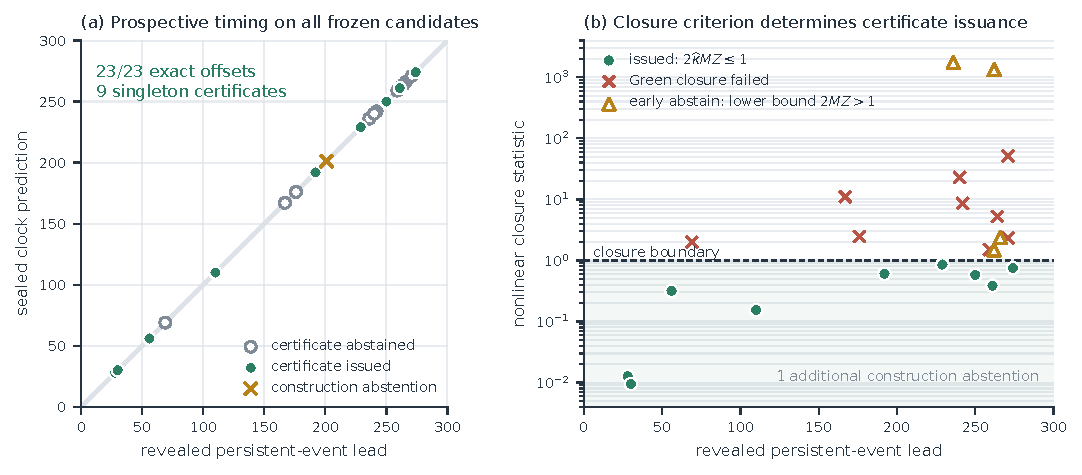
\includegraphics[width=\linewidth]{../figures/paper_transformer_green_confirmation.pdf}
  \caption{Prospective fixed-radius Transformer confirmation.  (a) Every one
  of the 23 prospectively selected clock events matches the revealed offset;
  filled points are the nine issued certificates.  (b) The nonlinear closure
  criterion determines certificate issuance.  Triangles are proof-preserving
  early lower bounds; one construction abstention has no statistic.}
  \label{fig:transformer-green}
\end{figure}

Table~\ref{tab:allfresh} reports every frozen candidate, including abstentions.
For Green-probed rows, ``stat.'' is $2\widehat\kappa MZ$; for early rows it is
the lower bound $2MZ$.  The construction row has no valid centerline and no
statistic.  Prediction and revealed lead agree in all rows.

\begin{table}[H]
\caption{Complete frozen fresh Transformer candidate audit.  ``Stat.'' is the
full Green closure for probed rows and its $\kappa\ge1$ lower bound for early
abstentions.}
\label{tab:allfresh}
\centering
\footnotesize
\setlength{\tabcolsep}{4.2pt}
\begin{tabular}{rrrrlr}
\toprule
Seed & Gate & Anchor & Lead & Disposition & Stat. \\
\midrule
331&70\%&1,160&262&early abstain&1.485\\
331&80\%&1,520&271&closure abstain&51.219\\
333&70\%&3,000&28&issued&0.013\\
333&80\%&3,080&192&issued&0.607\\
335&70\%&2,440&201&construction abstain&--\\
335&80\%&2,880&110&issued&0.154\\
335&90\%&3,240&229&issued&0.855\\
337&70\%&1,080&242&closure abstain&8.603\\
337&80\%&1,720&250&issued&0.580\\
342&70\%&1,480&69&closure abstain&1.996\\
345&70\%&960&236&early abstain&1,739.181\\
345&80\%&1,320&30&issued&0.009\\
345&90\%&2,120&261&issued&0.386\\
347&70\%&2,000&266&early abstain&2.362\\
348&70\%&2,200&56&issued&0.318\\
348&80\%&2,840&264&closure abstain&5.240\\
348&90\%&3,240&176&closure abstain&2.471\\
350&70\%&1,440&262&early abstain&1,331.466\\
350&80\%&2,920&274&issued&0.747\\
351&70\%&1,600&167&closure abstain&11.062\\
351&80\%&2,200&240&closure abstain&22.905\\
352&80\%&5,320&259&closure abstain&1.505\\
354&70\%&2,120&271&closure abstain&2.346\\
\bottomrule
\end{tabular}
\end{table}

The 72-case disposition is: 23 candidates, 29 causal screens with no future
modal candidate, 19 never eligible, and one gate already present.  Candidate
rate is 31.9\%; issuance is 12.5\% over all cases and 39.1\% conditional on a
candidate.  Candidate seeds are
\{331,333,335,337,342,345,347,348,350,351,352,354\}; issuing seeds are
\{333,335,337,345,348,350\}.

\section{Independent response-centered Transformer audit}
\label{app:v3-audit}

The method, candidate, and certificate seals have SHA-256 prefixes
\texttt{2CB9738FD630392C}, \texttt{43A016761DEB48CB}, and
\texttt{05D9FC835AEB58C8}.  The outcome audit prefix is
\texttt{E8BEEC6A28AC1AC3}.  The method seal precedes training seeds 355--378;
the candidate seal precedes every randomized query; and the certificate seal
precedes every future rollout.

\begin{table}[H]
\caption{All 19 independently frozen response-centered candidates.  ``q'' is
the first issuing shared-probe power; ``base'' is the matched power-8
fixed-radius rule.  Every finite centerline prediction equals the revealed
lead.}
\label{tab:v3-all}
\centering
\footnotesize
\setlength{\tabcolsep}{3.6pt}
\begin{tabular}{rrrrrrrr}
\toprule
Seed & Gate & Anchor & Lead & q & v3 & Base & Disposition \\
\midrule
360&70\%&3,480&107&3&yes&yes&issued\\
361&70\%&1,880&251&--&no&no&closure\\
361&80\%&2,800&265&2&yes&yes&issued\\
365&70\%&1,480&127&--&no&no&construction\\
366&70\%&1,040&28&2&yes&yes&issued\\
366&80\%&1,120&2&1&yes&yes&issued\\
366&90\%&1,360&70&2&yes&yes&issued\\
368&80\%&2,880&256&--&no&no&closure\\
369&70\%&4,160&157&2&yes&yes&issued\\
369&80\%&4,480&118&2&yes&yes&issued\\
369&90\%&5,760&232&2&yes&yes&issued\\
370&70\%&2,280&275&2&yes&yes&issued\\
372&70\%&3,440&246&4&yes&no&issued\\
373&70\%&1,280&247&--&no&no&closure\\
373&80\%&1,760&214&--&no&no&closure\\
375&70\%&920&217&--&no&no&early\\
375&80\%&1,800&118&3&yes&yes&issued\\
378&70\%&3,640&261&--&no&no&closure\\
378&90\%&4,800&138&--&no&no&early\\
\bottomrule
\end{tabular}
\end{table}

The 72-case disposition is 19 candidates, 42 trigger-visible screens with no
future modal event, and 11 never-eligible gates.  V3 issues 11/19 candidates
(11/72 cases) across seven seeds; the fixed-radius baseline issues 10/19.
Conditional coverage is 11/11 and 10/10, respectively.  First issuing powers
have counts $(1,7,2,1)$ for $q=(1,2,3,4)$.

Seed 365 exposes an implementation invariant rather than a favorable
exclusion.  The blind selector found an event on a truncated modal path, while
the constructor required every sweep to reach the full 300-step horizon.
Before outcomes, a hash-bound execution amendment retained the case in the
denominator as a zero-query abstention and prohibited retrying, shortening, or
changing the numerical cap.  Future selectors enforce the constructor's full
horizon invariant.

All 11 issued total-state radii contain the revealed trajectories.  The
stricter response-centered remainder diagnostic has 11 float64 violations at
machine scale; the maximum absolute radius deficit is
$3.07\times10^{-14}$.  Every bracket survives added state-radius padding
through $10^{-8}$ and all survive $10^{-7}$ (maximum width one), while only
two survive $10^{-6}$.  This records numerical headroom but does not infer an
outward error bound from observed discrepancies.

A separate 256-bit Arb audit treats each stored binary64 probe norm $Y$ as an
exact dyadic input, outward-encloses the folded-normal quantile and every
$(Y/c_\delta)^{1/(2q)}$ root, and takes the maximum with each stored bound.
The stored $c_\delta$ is already one ulp below the exact-quantile enclosure;
13,052 scalar rows require upward repair, with maximum factor
$1+8.9\times10^{-16}$.  All 11 brackets remain identical and minimum logic
slack is $1.80\times10^{-4}$ (audit SHA-256 prefix
\texttt{74B40EE5E10C19CE}).  HVP/VJP, norm accumulation, jets, and margins are
outside this conditional scalar audit.

The post-seal time-resolved theorem audit on seed 372 reduces the forcing term
to 67.5\% of the scalar value and the power-4 state radius from
$2.73\times10^{-14}$ to $2.06\times10^{-14}$.  Combining that theorem with a
role-stratified allocation of the unchanged $10^{-6}$ family budget closes the
same $[246,246]$ event at power three.  The audit file has SHA-256 prefix
\texttt{6B1084D07558AC0A}; it is method-development evidence and leaves the
sealed v3 disposition unchanged.

\section{Cancellation-safe second-response audit}
\label{app:two-response-audit}

Corollary~\ref{cor:directional-two-response} was implemented after the v3
seal without reading future trajectories.  The implementation contracts the
third derivative of the objective twice with the parameter component of
$\widetilde z_j$, propagates the resulting signed $q^{(2)}$ through one more
causal Green sweep, and reserves the local fourth-order Taylor bound plus
arithmetic residuals in Eq.~\eqref{eq:directional-two-response}.  It never
subtracts two nearly equal optimizer maps.

The adaptive policy first applies the prospective zero-extra closure.  If that
issues, it stops; if $bp\ge1$, no second-order forcing can repair the current
power, so it refines the shared Gram iterate.  Only when $bp<1$ and the
zero-extra forcing still fails does it construct $q^{(2)}$ and $\widetilde y$,
which are then reused at every later power.

\begin{table}[H]
\caption{Outcome-blind post-seal second-response audit.  Net HVPs subtract the
extra causal responses but exclude directional third-product cost.  The
amplified benchmark includes every branch-specific fourth-order envelope.  No
prospective disposition or coverage count changes.}
\label{tab:two-response-audit}
\centering
\small
\setlength{\tabcolsep}{8pt}
\begin{tabular}{lr}
\toprule
Quantity & Result \\
\midrule
Green-evaluable sealed records & 15 \\
Zero-extra / directional closures & 11 / 15 \\
Prior abstentions converted & 4 \\
Existing closures advanced & 5 \\
Adaptive invocations / no-added-work cases & 9 / 6 \\
Progressive power levels removed & 22 \\
Net objective HVPs removed & 167,250 \\
Directional third products added & 1,797 \\
Local fourth-order Taylor gates & 9/9 \\
Minimum Taylor headroom & $55.3\times$ \\
Paired branch / next-power median & 78.58 / 233.45 s \\
Paired speedup (four-pair range) & $2.91\times$ ($2.77$--$3.28\times$) \\
Amplified secant $\lambda$ / bracket & 4096 / $[28,28]$ \\
Secant / third-AD / next-power median & 6.56 / 8.10 / 26.01 s \\
Secant speedup vs. third-AD / next power & $1.19\times$ / $4.04\times$ \\
Secant analytic headroom & $24.4\times$ \\
Outward scalar jets / precision & 204 / 192 bits \\
Exact forcing bound / wall time & $1.31\times10^{-29}$ / 9.80 min \\
Response-free bracket / forcing headroom & $[28,28]$ / $24.41\times$ \\
Relinearized mixed coefficient & $0.627\to0$ \\
Relinearized 16-probe forcing headroom & $173.73\times$ \\
Four-probe bracket / forcing headroom & $[28,28]$ / $2.00\times$ \\
Relinearized Green applications & $16\to4$ \\
Four- / 16-probe median time & 6.51 / 23.64 s ($3.63\times$) \\
\bottomrule
\end{tabular}
\end{table}

At each invoked stopping power, the measured directional forcing is at most
$2.60\times10^{-13}$ of the zero-extra bound (median
$3.02\times10^{-15}$).  A separate deterministic scalar jet propagates
Transformer derivatives through order four.  Rather than charging a large
anchor ball to every parameter block, it evaluates the exact segment ball
$c_j+t\widetilde z_j$ checkpointwise.  All nine invoked cases satisfy the
analytic Taylor gate; headroom over $\sigma_2$ ranges from $55.3\times$ to
$1.80\times10^5$.  The independent structural audit reproduces all counts,
operator accounting, sealed Green domination, and fourth-order inequalities
(SHA-256 prefix \texttt{75A8FAA37DFC92EF}).  The remaining headroom is not
silently promoted to a proof: outward directional-product and recurrence
residual bounds are still required before this post-seal audit can become a
fresh computer-assisted Transformer certificate.

The incremental timing audit holds the centerline, first response, and first
Gram power fixed, then alternates one additional 16-probe Gram power with the
directional forcing plus scalar causal response.  On sealed seed 366 at the
70\% gate ($H=52$), all four checksums agree and every pair favors the
directional branch; the independent arithmetic/hash audit reads no future
outcome.  Absolute times were collected under concurrent workspace load, so we
interpret the within-pair ratio rather than claim a machine-independent latency.

Corollary~\ref{cor:amplified-secant} was then implemented with the fixed
power-of-two amplification $\lambda=4096$.  It evaluates one shifted gradient
and one existing HVP per checkpoint, divides the nonlinear numerator by
$\lambda^2$, and reserves the exact ray-secant discrepancy from
Eq.~\eqref{eq:amplified-secant}.  On the same sealed $H=52$ case it closes the
power-one $[28,28]$ bracket, while the analytic discrepancy consumes only
1/24.4 of the admissible injection-error budget; $6.01\times10^{-20}$ remains
for outward arithmetic and recurrence residuals.  Three rotating-order triples
time the secant, third-product, and next-power branches after identical shared
setup.  Their medians are 6.56, 8.10, and 26.01 seconds, respectively; every
pair favors the secant over the next power (range $3.82$--$4.37\times$).
An independent arithmetic/hash audit reproduces the bracket, closure,
headroom, checksums, and every timing ratio without reading a future outcome.
After a 16-probe development audit, a new protocol froze four fresh forcing
probes under a separate nonce.  A 192-bit Arb multi-jet evaluates attention,
exact GELU, softmax, cross-entropy, and weight decay while sharing each forward
pass across all four directions.  An adversarial audit caught a preliminary
binary64 subtraction in $w=g_w-g_\theta$; v2 preserved every probe and formed
that difference inside Arb.  Across all 51 checkpoints, its 204 outward
intervals bound the exact secant forcing by $1.31\times10^{-29}$, retain
$[28,28]$ with $24.41\times$ headroom, and take 9.80 minutes wall time (8.58
minutes for jets) on four workers.  Twelve randomized architecture-level tests
match PyTorch objectives, gradients, and mixed products within
$6.67\times10^{-16}$; an independent interval/hash audit re-sums every row.
This closes the scalar secant obligation conditional on stored dyadic inputs,
not the upstream Transformer arithmetic or prospective evidence boundary.

\paragraph{Corrected-path Green audit.}
We next froze a rebuilt Green operator on the corrected center
$b=c+\widetilde z$.  The first protocol evaluated
$G(b_j)-b_{j+1}$ literally in float64; cancellation inflated the measured
forcing norm to $3.10\times10^{-15}$ and produced a negative discriminant.
We retain this failed interface.  A second, separately frozen protocol instead
used Eq.~\eqref{eq:corrected-defect-identity} with the amplified secant, so it
never subtracts nearly equal optimizer maps.  With 16 fresh probes at power
one, it removes the old mixed coefficient $0.6273518$, obtains
$173.73\times$ injection-forcing headroom, and retains $[28,28]$ without a
second causal response.

That slack motivated one prespecified four-probe reduction, frozen before its
new Gaussian block.  The resulting Green bound is looser
($\bar\kappa=45015.33$), yet the corrected closure retains $[28,28]$ with
$2.0028\times$ forcing headroom and a total radius
$2.86\times10^{-15}$.  An independent outcome-blind auditor regenerates all
four Gaussian vectors, $\bar K_H^\top\bar K_H$ products, calibration, scalar
root, margins, and bracket.  The logical Green block falls from 16 to four
applications.  Three alternating matched pairs give medians 6.51 versus
23.64 seconds, or $3.63\times$ (pairwise range $3.48$--$4.10\times$), with
shared centerline setup excluded.  These post-seal audits do not alter the
prospective cohort.  The scalar secant forcing is outward conditional on stored
dyadic inputs; response recurrence, rebuilt Green products, derivative
envelopes, and output margins remain float64/high-confidence rather than a
complete computer-assisted Transformer proof.

We then froze a cohort-wide release over all 15 Green-evaluable v3 records,
before drawing its Gaussian block and without reading outcomes.  It combines
the corrected center, prefixes $m\in\{4,8,16\}$, one Gram power, and equal
family spending.  Every record issues the same bracket as the sealed
directional baseline: 14 stop after four probes and one after eight.  Relative
to that baseline, the Green block contracts from 560 to 64 Gram applications
($8.75\times$); including the response/replay accounting declared by each
protocol, the theoretical linearized schedule contracts from 1,150 to 144
sweeps ($7.99\times$).  The minimum forcing headroom is $2.293\times$ and the
minimum strict event-logic slack is $1.45\times10^{-6}$.

This is the complete pre-existing operator cohort, not a pass-selected subset.
Each of the other four among 19 frozen candidates failed the original
deterministic pre-query screen, so the frozen protocol instantiated no Green
operator on which a probe-count replay could be defined.

The new Green family spends $10^{-6}$ and the inherited output family spends
at most $10^{-6}$, giving the explicit combined upper bound $2\times10^{-6}$.
An independent auditor regenerates all 64 unique Gaussian vectors and
recomputes every operator, root, closure, margin, hash, and bracket.  Direct
image screening under the same Gaussian event issues four cases before a
transpose; Gram fallback issues the other 11.  It therefore avoids 16 of 128
staged probe sweeps (128 to 112, $1.143\times$), a useful but deliberately
separate gain from the larger corrected-prefix reduction.

The scaled-momentum factorization in
Corollary~\ref{cor:parameter-forcing} permits a smaller operator without
changing the reference path or output rule.  A post-v1.0.1 protocol fixed
$T_\theta=\Pi_\theta\bar K_H\mathcal B$, the same 4/8/16 direct/Gram policy,
a fresh nonce, and a new $10^{-6}$ Green-family budget before drawing any
probe.  It preserves all 15 inherited brackets, with six direct-image and nine
Gram releases, and reduces the staged total from 112 to 96 logical sweeps
($1.167\times$).  An independent mechanical verifier checks all 17 sealed
dependency hashes and 15 caches and recomputes every stored Gaussian bound,
quadratic root, bracket, and aggregate.

An adversarial proof audit then made the causal indexing explicit:
$\bar K_H$ returns $(e_1,\ldots,e_H)$ while update $j$ uses $e_j$.  The
earlier scalar bound remains valid because the shift in
Eq.~\eqref{eq:anchor-shift} has norm one.  A separately sealed follow-up
removed the identically zero update-zero forcing block as prescribed by
$Q_0$.  All 15 brackets again survive, but the total remains 96 sweeps (median
selected randomized gain-bound ratio $0.994$), so the prespecified
strict-improvement gate fails.  We report this negative result because it both
validates the corrected indexing and locates the remaining bottleneck: coarse
randomized release thresholds, not the zero anchor block.

Finally, Proposition~\ref{prop:causal-prefix} is executable rather than only
an accounting identity.  Three natural Transformer records reproduce the
full-$H=300$ centerline bitwise at sealed horizons 26, 131, and 299, including
the same persistent-event prediction.  Prefix streaming reduces centerline
time by $9.94\times$, $2.09\times$, and $1.06\times$, and estimated path
storage by $39.6\times$, $10.5\times$, and $4.84\times$, respectively.

Corollary~\ref{cor:analytic-jet-release} was then replayed on the same complete
15-case operator cohort.  The deterministic screen alone issues eight cases
with the same singleton brackets, while the existing output-probe path handles
the other seven; staged issuance therefore remains 15/15.  Those eight releases
remove 1,432 randomized output-Jacobian operators and 22,912 $q=1$ Gram
applications.  Their maximum analytic margin radius is
$4.56\times10^{-10}$ against minimum strict logic slack
$1.80\times10^{-4}$, and their probability upper is only the $10^{-6}$ Green
event.  The audit reads zero outcome files.  A separately implemented replay
recomputes all analytic drift constants, quadratic roots, anchor margins, and
event brackets and reproduces 8/15 exactly.

\begin{table}[H]
\caption{Frozen, outcome-blind corrected-prefix release over every
Green-evaluable v3 record.  The staged direct/Gram audit reuses the same
Gaussian event, so it adds no failure probability.  These are post-seal
mechanism and implementation results, not additional prospective coverage
counts.}
\label{tab:prefix-panel}
\centering
\small
\setlength{\tabcolsep}{8pt}
\begin{tabular}{lr}
\toprule
Quantity & Result \\
\midrule
Evaluated / issued / preserved brackets & 15 / 15 / 15 \\
Stopping prefix $m=4/8/16$ & 14 / 1 / 0 \\
Green Gram applications & $560\to64$ ($8.75\times$) \\
Declared linearized sweeps & $1{,}150\to144$ ($7.99\times$) \\
Pairwise Green reduction, median (range) & $8\times$ ($4$--$16\times$) \\
Minimum forcing headroom & $2.293\times$ \\
Direct-image / Gram-fallback routes & 4 / 11 \\
Staged probe sweeps & $128\to112$ ($1.143\times$) \\
Full-state / parameter-forcing staged sweeps & $112\to96$ ($1.167\times$) \\
Anchor-zero refinement versus parameter forcing & $96\to96$ (gate failed) \\
Deterministic-jet / output-probe routes & 8 / 7 \\
Randomized output operators eliminated & 1,432 \\
Output $q=1$ Gram applications eliminated & 22,912 \\
Streaming time reduction, $H=26/131/299$ & $9.94/2.09/1.06\times$ \\
Streaming storage reduction, $H=26/131/299$ & $39.6/10.5/4.84\times$ \\
Combined failure-probability upper bound & $2\times10^{-6}$ \\
Minimum strict event-logic slack & $1.45\times10^{-6}$ \\
Outcome files read & 0 \\
\bottomrule
\end{tabular}
\end{table}

\begin{figure}[H]
  \centering
  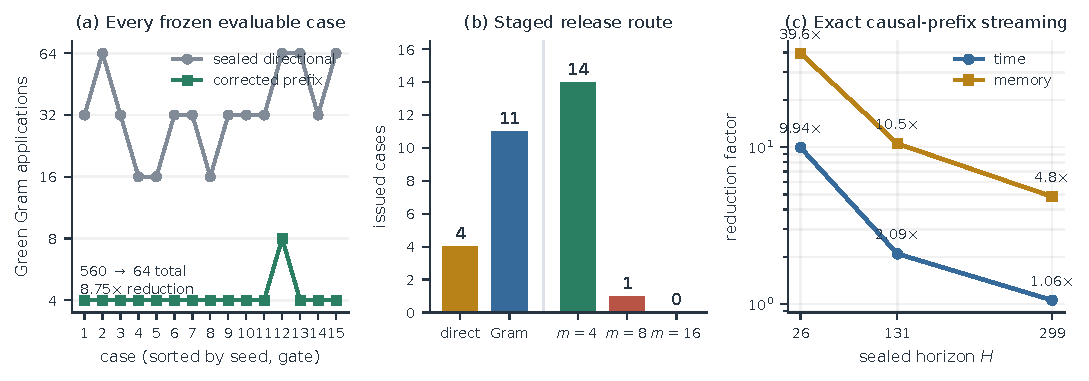
\includegraphics[width=\linewidth]{../figures/paper_relinearized_prefix_panel.pdf}
  \caption{Practical effect of corrected-path, prefix-local release.
  (a) Every frozen evaluable case preserves its bracket with fewer Green Gram
  applications.  (b) Direct images issue four cases before a transpose; most
  still require the sharper Gram release.  (c) Causal streaming is bitwise
  identical to the full path and pays only for the sealed horizon.}
  \label{fig:prefix-panel}
\end{figure}

The execution ledger preserves two deviations.  An initial smoke execution
double-counted a pending block, generated and applied two vectors, and then
errored before producing any prefix statistic, result, or cache; that nonce was
discarded and the corrected loop was frozen under a fresh nonce.  In one v2
case, a later norm-only issuance short-circuited before a cached direct response
was reused.  This was conservative: the stored bound exceeds the latent
direct-aware bound by $1.11\times10^{-8}$ relatively, and no disposition,
prefix, or bracket changes.  Both events and their hashes remain in the
supplement rather than being silently repaired.

\section{Directional block remainder and mixed-jet audit}
\label{app:block-directional-audit}

The post-release audit froze the 15-case corrected-path cohort, disclosed
seed 366 at the 80\% gate as the development row, and reserved the other 14
cases for the promotion decision.  It changed only the fourth-order Taylor
term: centerlines, three-sweep corrections, domain radii, recorded
family-calibrated Green bounds, drift constants, and event logic were inherited
unchanged.  No future-outcome file was read and no new Gaussian vector was
drawn.

For the one-block Transformer, the analytic partition has 14 orthogonal blocks:
joint token/position embedding; separate query, key, and value weight/bias
blocks; attention output weight/bias; two feed-forward weight/bias pairs; and
the readout.  Nonnegative derivative polynomials are propagated through
attention, GELU, softmax, and cross entropy.  Segment values are inflated by a
monotone first-order fixed point before the fourth-order majorant is evaluated.
Product/chain-rule scalarization, exact partition, Euler homogeneity, and 12
direct mixed-fourth autodiff tests all pass.

\begin{table}[H]
\caption{Frozen directional-block audit.  ``New'' means closure under the
three-sweep rule where the scalar fourth-order comparator abstains; all event
brackets already belong to the sealed four-sweep cohort and are not counted as
new prospective coverage.}
\label{tab:block-directional-audit}
\centering
\small
\setlength{\tabcolsep}{8pt}
\begin{tabular}{lr}
\toprule
Quantity & Result \\
\midrule
Cases / nondevelopment cases & 15 / 14 \\
Directional/scalar ratio, holdout median & $3.45\times10^{-4}$ \\
Holdout tightening, median (range) & $2{,}899\times$ ($977$--$10{,}997\times$) \\
Three-sweep closures, scalar / directional & 1 / 4 \\
New nondevelopment closures & 3 \\
Issued / sealed bracket retained & 4/4 / 4/4 \\
Issued offsets & 2, 28, 70, 118 \\
Minimum strict event slack & $1.36\times10^{-3}$ \\
Every checkpoint no weaker than scalar & yes \\
Independent mixed-jet maximum relative error & $4.19\times10^{-15}$ \\
Polynomial / mixed-jet median runtime & 154.31 / 115.92 s \\
Whole-case runtime ratio / frozen gate & $1.33\times$ / $2\times$ (failed) \\
Outcome files / new randomized queries & 0 / 0 \\
\bottomrule
\end{tabular}
\end{table}

\begin{figure}[H]
  \centering
  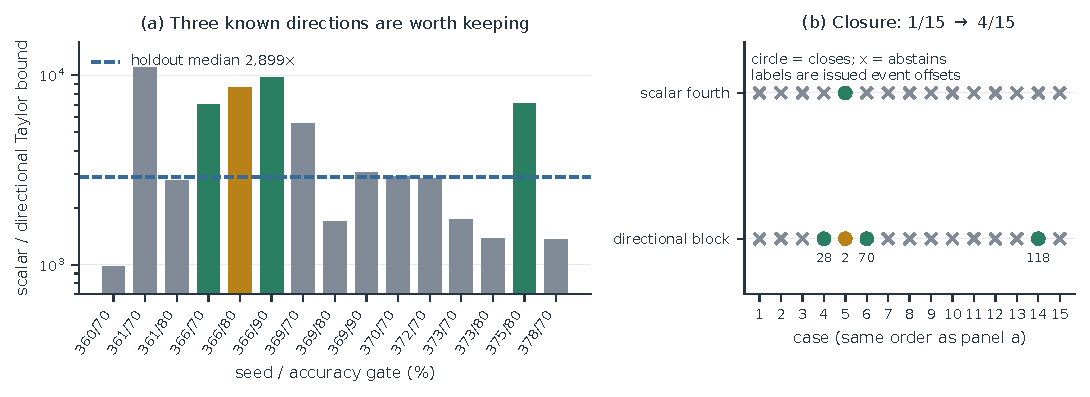
\includegraphics[width=\linewidth]{../figures/paper_directional_block_remainder.pdf}
  \caption{Directional fourth-order geometry in the complete frozen panel.
  (a) Scalar-to-directional Taylor tightening; green bars are new holdout
  closures, ochre is the disclosed development row, and gray cases still
  abstain.  (b) The scalar rule closes one case, whereas the directional rule
  closes four and returns the labeled sealed offsets.}
  \label{fig:block-directional-audit}
\end{figure}

The independent implementation does not differentiate the stored polynomial.
It propagates a bivariate jet in a known variable $t$ and a free block variable
$\varepsilon$, retaining $D_t^k$ and $D_t^kD_\varepsilon$ for $k\le3$.
Across all 15 cases it reproduces every local Taylor bound and closure decision.
Its prespecified $2\times$ whole-case speed gate fails at $1.33\times$ because
centerline replay remains dominant.  This negative timing gate is part of the
result: the practical saving established here is one fewer predeclared
centerline sweep on four records, not a twofold acceleration of the complete
verifier.

\section{Matched unsigned baseline and sweep audit}
\label{app:mechanism}

The unsigned comparator keeps the same causal Green operator and therefore the
same finite-window conditioning information.  It changes only the zero-order
response:
\begin{equation}
 Z=\norm{K_Hs}
 \quad\longrightarrow\quad
 Z_{\rm u}=\kappa\norm{s}.
\end{equation}
For its own ball it solves the radii polynomial
\begin{equation}
 p_{\rm u}(R)=Z_{\rm u}+\tfrac12\kappa M(R)R^2-R\le0
\end{equation}
and chooses the smallest admissible root.  The analytic neural envelope is
coordinatewise nondecreasing in $R$.  Thus, whenever
$Z_{\rm u}>2Z$, every admissible unsigned radius contains the frozen signed
ball, and evaluating the unsigned closure with the smaller signed-ball
$M(2Z)$ is already favorable to the baseline.  Failure of that lower envelope
proves failure at every admissible unsigned radius.  This argument eliminates
17/18 matched cases without numerical reconstruction.  The remaining case,
seed 345 at the 80\% gate, is reconstructed with its own outer-ball jet and
retains $[30,30]$; it is the baseline's sole issued certificate.

\begin{table}[H]
\caption{Complete 0--4-sweep audit on the three sealed burned-development
candidates.  Defect is the median across candidates of the maximum scaled path
defect.}
\label{tab:sweeps}
\centering
\small
\setlength{\tabcolsep}{7pt}
\begin{tabular}{rrrrr}
\toprule
Sweeps & Cumulative HVPs & Exact clocks & Median $|$error$|$ & Defect \\
\midrule
0 & 300   & 0/3 & 3 & $8.57\times10^{-3}$ \\
1 & 600   & 3/3 & 0 & $2.23\times10^{-3}$ \\
2 & 900   & 3/3 & 0 & $5.85\times10^{-4}$ \\
3 & 1,200 & 3/3 & 0 & $2.58\times10^{-5}$ \\
4 & 1,500 & 3/3 & 0 & $5.94\times10^{-8}$ \\
\bottomrule
\end{tabular}
\end{table}

The median incremental construction times for stages zero through four are
26.56, 24.58, 31.04, 34.70, and 37.15 seconds.  These are diagnostic timings,
not a fresh model-selection study.  Their role is to expose the numerical
mechanism behind the prospectively fixed choice of four sweeps.

\section{Matrix-free scaling accounting}
\label{app:scaling}

For $H=300$, four sweeps require 1,500 objective HVPs.  The frozen
$m=16,q=8$ Green probe requires 76,800 objective HVPs, and the output-margin
probe requires 38,528 output-Jacobian Gram products.  These are logical calls:
the batched implementation evaluates the same 16 independent rows together,
preserving their generation order, $Y$ maximum, calibration, and union budget.
Tests compare HVP, optimizer JVP/VJP, causal Green, transpose, output-Gram, and
the final probabilistic bound against scalar execution; maximum relative error
is $3.24\times10^{-16}$.

\begin{figure}[H]
  \centering
  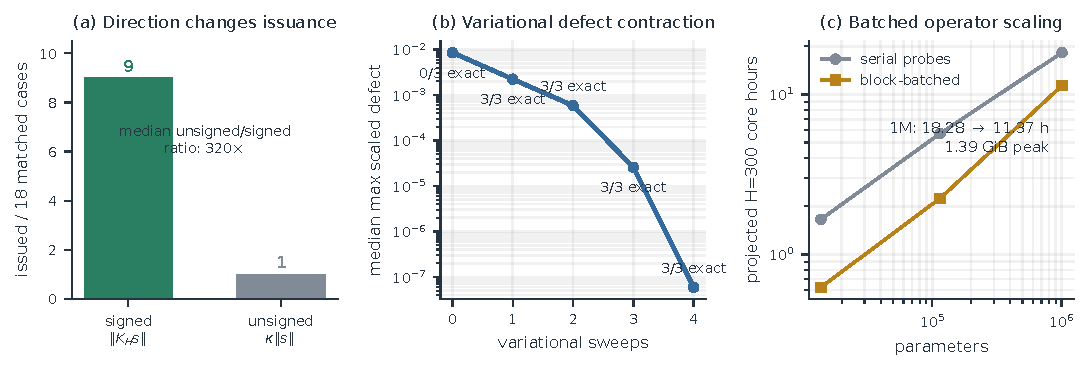
\includegraphics[width=\linewidth]{../figures/paper_mechanism_scaling.pdf}
  \caption{Mechanism and scale.  (a) The matched scalar Euclidean unsigned
  finite-window baseline retains only 1/9 signed Transformer certificates;
  direction removal inflates the zero-order term by a median $320\times$.
  (b) Variational sweeps rapidly contract the known path defect; one sweep
  already makes all three burned-development clocks exact.  (c) Evaluating the
  same 16 probes as one reverse-mode block lowers the matched $H=300$ core
  projection at every tested width.}
  \label{fig:mechanism-scaling}
\end{figure}

\begin{table}[H]
\caption{Matched serial-versus-block-batched projection for the unchanged full
$H=300$, four-sweep, $m=16,q=8$ core.  Both columns use same-run timings and
exclude jets, orchestration, I/O, and cache effects.}
\label{tab:scale}
\centering
\small
\setlength{\tabcolsep}{5.0pt}
\begin{tabular}{rrrrr}
\toprule
Params & Serial core & Batched core & Speedup & Peak GiB \\
\midrule
13,792    & 1.66 h & 0.62 h & $2.66\times$ & 0.36 \\
115,104   & 5.70 h & 2.24 h & $2.54\times$ & 0.53 \\
1,008,864 & 18.28 h & 11.37 h & $1.61\times$ & 1.39 \\
\bottomrule
\end{tabular}
\end{table}

Table~\ref{tab:scale} uses serial and batched block timings from the same run.
An earlier isolated-one-product multiplication yielded 6.16/18.98/65.88 hours;
the JSON record retains it for traceability, but it is not used as the speedup
denominator because same-run serial blocks are materially faster.  Both
projections exclude jets, Python orchestration, checkpoint I/O, and cache
effects.  At 1,008,864 parameters the batched 16-direction HVP and output-Gram
blocks are $1.58\times$ and $1.79\times$ faster, with 1.39\,GiB process peak.

For a direct wall-clock baseline, the historical frozen fixed-$q=8$ paper
batch has 22 candidate constructions taking 19.44 aggregate hours and a median
of 58.02 minutes, whereas continuation of 300 actual updates estimated from all
24 training traces takes a median of 5.31 seconds ($655.8\times$ less).  Those
numbers describe the original implementation, not the composed verifier.
On the sealed seed-366 80\% case, three separately launched executions combine
exact prefix streaming, one signed corrected-path sweep, deterministic neural
jets, and a four-probe direct-image release.  All reproduce $[2,2]$ in
9.01--11.71 seconds (median 9.21), with four forward Green applications, zero
transpose applications, zero randomized output operators, and family failure
upper $10^{-6}$.  Relative to the historical cross-batch median this is an
$378\times$ reduction.  A same-machine three-repeat control measures direct
continuation at 0.298 seconds for the required 26 updates and 3.718 seconds for
300, leaving certification $30.9\times$ and $2.48\times$ slower.  Continuation
computes the future outcome; \method{} constructs an outcome-independent proof object
before that trajectory is opened.  On the small exact-real WDBC audit,
where validated continuation is
the matched proof baseline rather than an ordinary rollout, the direction
reverses: 7.12 hours for direct continuation versus 33.88 minutes for the
GreenCert records (Table~\ref{tab:wdbc-direct}).

Two end-to-end replays rebuild all four sweeps, analytic envelopes, output
logic, and the Green probe from the sealed checkpoint and committed streams.
Seed 333's $[28,28]$ certificate falls from 17.82 to 5.94 minutes
($3.00\times$); seed 345's $[30,30]$ falls from 17.34 to 6.66 minutes
($2.60\times$).  Maximum disagreement in any bound or closure statistic is
$2.14\times10^{-16}$, and both dispositions are unchanged.

The witness-sparse audit reconstructs every one of the 11 response-centered
brackets from its $K$ certified success times and a greedy minimum-cardinality
set of certified failures.  Event-query times fall by a median
$4.73\times$ (range $1.00$--$8.31\times$).  Replacing the current all-289-input
output operator by transition-state training operators (173 examples) and
witness-state certification operators (58 examples) gives the exact
example-level accounting
\((H-1)173+|W|58\), a median 36.3\% reduction relative to \(H\cdot289\).
The predictable acquisition policy then discovers all 11 witness sets from
raw centerline slacks and prior query results, reducing 1,882 full-time queries
to 349 (audit SHA-256 prefix \texttt{1AEA107F9EFF5C5}).  A matched timing panel
at horizons 26, 52, 94, and 142 preserves all four sealed brackets without
fallbacks.  Direct-sum role fusion reduces aggregate example-pair work 33.7\%
and gives $1.37\times$ operator and $1.35\times$ output-wall speedups (range
$1.19$--$1.40\times$); including shared centerline time gives $1.11\times$.
The independent panel audit has SHA-256 prefix
\texttt{E35B1DD723371F86}.

A first monolithic replay composes online Green stopping with role-fused output
transport on the sealed $H=26$ case.  It keys witnesses to the frozen
centerline event, stops both operator families at $q=1$, uses no fallback, and
retains $[2,2]$.  Pair work falls 22.37\% and the same-process output-operator
wall time improves $1.29\times$; the matched complete replay improves only
$1.018\times$ (95.79 seconds measured), because centerline construction and
the Green solve dominate this short horizon.  This directly identifies the
remaining systems bottleneck rather than extrapolating output-only speedups
(record SHA-256 prefix \texttt{006CC711EDA43CC4}).

The final composition removes those two bottlenecks rather than combining
their isolated speedup factors.  Prefix streaming constructs only the required
26 checkpoints; corrected-path direct-image release stops after four forward
queries; and Corollary~\ref{cor:analytic-jet-release} replaces every randomized
output query by the already required ball-valid jets.  Median phase times over
the three fresh processes are 5.226\,s (centerline), 1.119\,s (signed correction),
0.678\,s (jets), 2.007\,s (Green), and 0.082\,s (closure and event logic), with
9.206\,s median end to end.  The independent audit record has SHA-256 prefix
\texttt{664993E294AD6010}.

Proposition~\ref{prop:inexact-probe} also yields an explicit numerical contract.
On that same $q=1$ replay, simultaneous verified Gram residuals
$\xi\le0.5999\widetilde Y$ for every Green/output query still retain the
singleton bracket (operator-bound inflation $1.2649\times$).  Green-only and
output-only tolerances are 4.2295 and 0.9107 times their terminal norms.  These
are admissible-residual sensitivities, not estimates of floating-point error.
A 50--50 max-column/chi-block confidence split additionally reduces the state
radius from $2.1331\times10^{-15}$ to $2.0705\times10^{-15}$ from the same
probe block and with no additional Gram application.

An actual mixed-precision replay then evaluates every committed $q=1$
Green/output Gram product in float32 and measures its discrepancy against the
binary64 target.  The largest observed residual ratio is
$3.36\times10^{-7}$, $1.79\times10^6$ below the common admissible threshold;
the residual-corrected outward scalar roots retain $[2,2]$ with only
$1+2.75\times10^{-8}$ Green-bound inflation.  Across four separately launched
five-repeat alternating-order runs, all 20 paired q=1 kernel speedups exceed
one; their pooled median is $1.83\times$ (range $1.04$--$2.38\times$;
invocation medians $1.66/1.86/1.89/1.78\times$).  These discrepancies are measured rather than outward-enclosed,
so the replay demonstrates concrete mixed-precision headroom, not a completed
exact-real neural-kernel proof (aggregate-audit SHA-256 prefix
\texttt{7E5619D0B9EE6A41}).

Finally, the output-recentering corollary is audited without opening any future
trajectory.  Across the 15 Green-evaluable response-centered records, its
proof-preserving intersection with the original enclosure retains 11/11 issued
certificates at identical powers and brackets.  The recentered output radii
have maximum ratio 0.091--0.602 at issuance (median 0.365), with no added random query.  No
abstention converts and no power decreases on this cohort; the measured gain is
strictly smaller output uncertainty and precision headroom.

For architectural transport, a separate profile uses two pre-LayerNorm blocks,
102,400 parameters, and a standard bias-corrected AdamW state of dimension
307,200.  The analytically derived optimizer JVP/VJP uses one neural HVP and
agrees with full autograd to below $9\times10^{-18}$ on an explicit test;
optimizer and horizon-3 Green adjoint errors at profile scale are
$5.45\times10^{-15}$ and $4.40\times10^{-15}$.  This establishes matrix-free
linear transport only, not the global LayerNorm/AdamW jets needed for closure.

\ifdefined\arxivversion\else
\section{Object-level literature comparison}

\begin{table}[H]
\caption{Representative method-level comparison; this is not a taxonomy of all
validated dynamics.}
\label{tab:novelty}
\centering
\footnotesize
\setlength{\tabcolsep}{3.0pt}
\begin{tabular}{>{\raggedright\arraybackslash}p{0.21\linewidth}>{\raggedright\arraybackslash}p{0.23\linewidth}>{\raggedright\arraybackslash}p{0.24\linewidth}>{\raggedright\arraybackslash}p{0.22\linewidth}}
\toprule
Representative method & State/object & Uncertainty or correction & Delivered claim \\
\midrule
Chow--Lin--Palmer;\newline Chow--Palmer \citep{chow1989shadowing,chow1992numerical}
& semilinear or finite numerical pseudo-orbit
& right-inverse/Newton correction
& existence of a shadowing orbit and proximity bound \\
Lessard--Reinhardt \citep{lessard2014rigorous}
& Chebyshev coefficient sequence for an IVP
& residual and radii polynomial
& rigorous solution existence/error enclosure \\
AutoBound/SafeRate \citep{streeter2022autobound}
& one optimizer step
& Taylor-remainder majorizer
& certified loss decrease \\
YES training bounds \citep{yeganegi2024yes}
& layerwise data/output mappings
& comparison with linear and intermediate baselines
& online training-quality and loss bounds \\
Abstract Gradient Training \citep{sosnin2026agt}
& reachable training-parameter sets
& training-data perturbation set
& robust prediction after training \\
Barrier robustness \citep{taheri2026barc}
& family of poisoned training trajectories
& learned barrier and scenario bound
& terminal poisoning-robustness radius \\
Adaptive SGD stopping \citep{aolaritei2026stopping}
& strongly convex stochastic trajectory
& time-uniform confidence sequence
& distance/suboptimality stopping certificate \\
CT-BaB \citep{shi2026ctbab}
& neural controller and input region
& verification-aware branch and bound
& post-training Lyapunov stability \\
Certified neural dynamics \citep{wicker2021iterative,mathiesen2026certified}
& learned/Bayesian dynamical model
& model or transition uncertainty
& reachability or surrogate-trajectory enclosure \\
Weight-space robustness \citep{weng2020weight}
& fixed trained network
& exogenous parameter ball
& robust prediction at that network \\
\method{}
& unique optimizer orbit from a realized anchor
& signed temporal defect plus nonlinear tube
& persistent empirical first-passage bracket or abstention \\
\bottomrule
\end{tabular}
\end{table}
\fi

\section{Dense outward and disjoint HVP details}

In the dense mod-11 study, all eight fresh models fit training.  Among 40
seed-gate pairs, 37 events occur and the chronological rule selects 27 anchors.
The uncorrected \vone{} tube issues 6/27 certificates; one-sweep recentered
\vtwo{} issues 16/27, loses none of the six, and contains all 16 crossings.
Median capped state horizon moves from 26 to 174 updates; 13/27 recentered tubes
reach the full 250-step window.  Fourteen brackets are singletons; the other two
are $[18,20]$ and $[64,70]$, containing leads 18 and 66.  All issued brackets
survive a separate 192-bit outward pass unchanged.

The mod-13 HVP study uses widths 48, seeds 202--205, and disjoint
train/trigger/certification sets of 101/34/34.  Of 20 seed-threshold cases, 19
become eligible; 13 gates are already present, four screens find no future
candidate, and two candidates remain.  Both issue persistent singleton
brackets, $[31,31]$ and $[4,4]$, and both cover.  They come from one seed.  No
dense Hessian entry is formed; the two-radius uncertainty certificate uses a
rank-64 active subspace and a declared family-wise probe failure probability
$4.2\times10^{-7}$.

\begin{figure}[H]
  \centering
  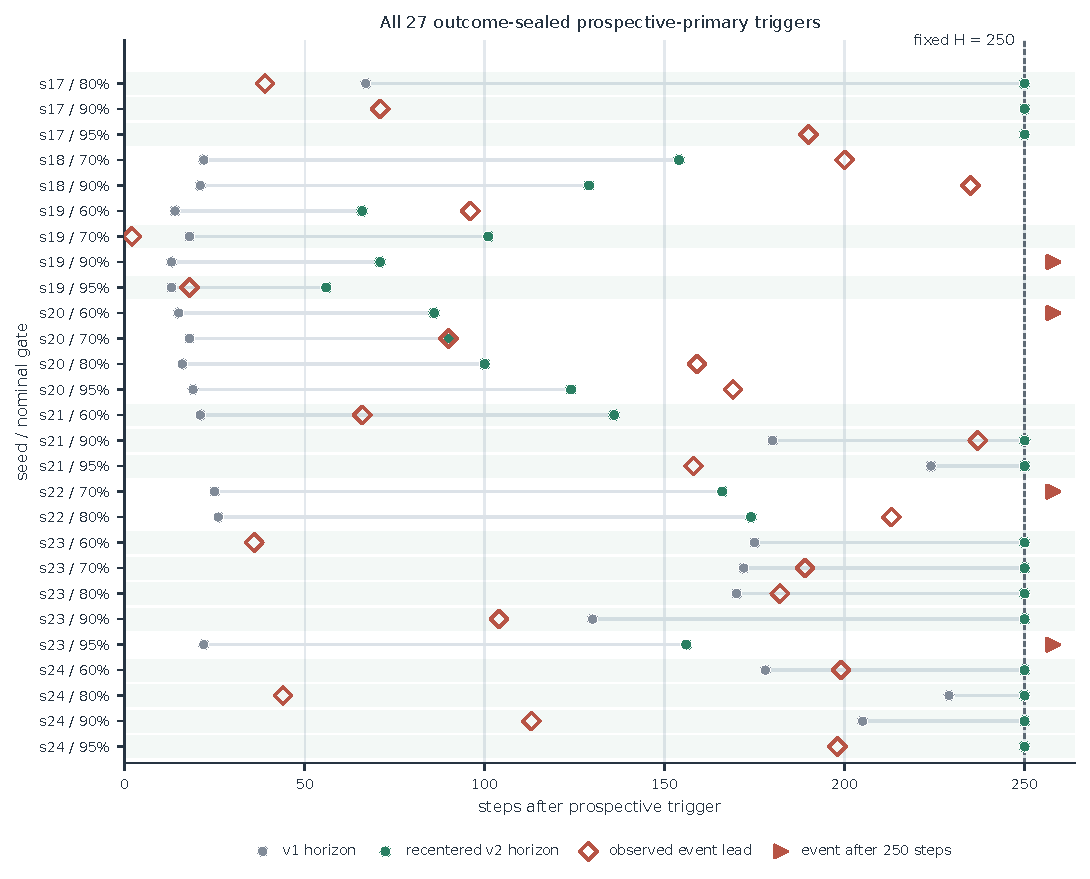
\includegraphics[width=0.92\linewidth]{../figures/paper_prospective_horizons.pdf}
  \caption{All 27 outcome-sealed dense triggers.  Signed recentering (teal) extends
  the median capped rigorous horizon from 26 to 174 updates relative to the
  norm-only baseline (gray).  Diamonds are observed event leads; triangles lie
  beyond the fixed 250-step window.}
  \label{fig:dense-horizons}
\end{figure}

\section{Numerical and reproducibility record}

\paragraph{Fixed-radius Transformer chain.}
The Transformer method, candidate manifest, pre-outcome certificate seal, and
final aggregate have SHA-256 prefixes \texttt{14EABFDE3823E228},
\texttt{D61FDFA72DAC8D70}, \texttt{4B6EBBAA877280F6A}, and
\texttt{A3D480FB92BFEC89}, respectively.  Complete hashes and a manifest of
every claim-bearing artifact are included in the supplement.

An independent checker does not import aggregation helpers.  It reloads all 23
certificate and post-seal audit files, verifies their hashes, recomputes
$R=2Z$, both closure inequalities, every 25-step persistent bracket from the
guaranteed/possible count arrays, the randomized budget, all coverage fields,
and seed-clustered summaries.  All checks pass.  Unit tests compare causal
Green products with an explicit block matrix, verify the real Transformer
adjoint, check the Gram exponent $1/(2q)$, finite-difference the scaled momentum
JVP, and enforce that candidate screening cannot read outcomes or make
probabilistic queries.  Random-direction jet tests are debugging checks only;
Appendix~\ref{app:transformer-jet} provides the line-by-line global analytic
derivation.  A separate exact-graph regression verifies that the sealed
bias-free-readout relaxation adds exactly one nonnegative first-degree
monomial and no second- or third-degree term.

\paragraph{Response-centered Transformer chain.}
The v3 method, candidate, certificate, and outcome-audit SHA-256 prefixes are
\texttt{2CB9738FD630392C}, \texttt{43A016761DEB48CB},
\texttt{05D9FC835AEB58C8}, and \texttt{E8BEEC6A28AC1AC3}.  The single
construction exception is separately bound by pre-outcome amendment seal
\texttt{66C452C64FBBBA75}.  Independent aggregation verifies all 72
dispositions, 19 modal predictions, 11 issued brackets, the matched 10-case
baseline, all first-issuing powers, 3,649 queried operators, and the realized
union bound.  Exact nonlinear scalar tests cover the response-centered and
time-resolved quadratic roots; resumable Gram tests reproduce every stored
power row from the same committed probe state.

\paragraph{WDBC chain.}
The complete hashes appear in Appendix~\ref{app:wdbc}.  Its selector test
attempts forbidden certification-set accesses and requires each to fail.
Candidate and certificate seals are verified before the independent outcome
join.  A second auditor that does not import the runner's aggregation code
reconstructs all 72 dispositions and all 56 brackets.  The direct-baseline
audit additionally checks that the outward recurrence contains no Green,
$\kappa$, probe, or random variable and verifies all 40 cached zero-radius
anchor tubes.

\paragraph{Digits chain.}
The raw scikit-learn arrays, protocol code, fresh seed list, and all constants
are committed by method seal \texttt{9901CD1A0E3FEABF}.  Loader tests prove
that training/selection cannot return certification tensors.  Candidate seal
\texttt{BFA31D77050F164D} fixes all 24 coordinates; certificate seal
\texttt{99AC9C628AFB4FC9} records 7/6/1 signed/unsigned/signed-only issuance
before outcome reconstruction.  A separate auditor that does not import the
runner recomputes all 24 anchors, checks every seal and event, and confirms
7/7 coverage; checkpoint reconstruction error is zero.  A second independent
audit verifies all seven 192-bit direct tubes, cache hashes, positive logic
slacks, exact bracket identity, and the signed-only $[147,147]$ event.  A
post-seal selectivity auditor independently identifies the two inaccurate
finite centerlines and verifies that both records are deterministic early
abstentions with no randomized query.

\paragraph{Post-seal hardening chain.}
The batched-operator tests compare every matrix-free product with scalar
evaluation.  Two complete replay records point to immutable original
certificate hashes and reproduce their centerlines, bounds, closures, and
brackets.  A separate aggregator recomputes all timing ratios and
million-parameter projections, verifies the digits outward caches without
importing their runner, and checks source hashes and adjoint identities for the
LayerNorm/AdamW primitive audit.
The matched anytime benchmark binds the original certificate and script hashes,
reproduces the $[2,2]$ decision with zero trace deviation, and records both
online and forced-q8 executions.  The time-resolved/role-budget audit uses only
sealed v3 traces and explicitly marks the prospective issuance result
unchanged.  The witness-sparse audit reconstructs all 11 issued first-passage
brackets, and 37,000 brute-force interval instances verify the greedy minimum
witness algorithm.  A second policy test covers 15,875 exhaustive and 2,000
randomized acquisition cases; its v3 replay reconstructs all 11 brackets using
only predictable queries.  Candidate-generic independent role-fusion audits
bind each sealed certificate, centerline, benchmark, and complete cache; they
reproduce four brackets with zero trace discrepancy and no fallback.  The
panel aggregator recomputes query counts, pair work, partial-phase timings,
and the naive-versus-fused comparison without importing the benchmark runner.
The 256-bit Arb audit encloses calibration and scalar roots conditional on
stored $Y$; an independent script rechecks its exact interval, certificate
hashes, and 11 retained brackets.  A strict post-fixed Transformer wrapper has
a fast
anchor-state regression and a complete 26-state audit on the shortest issued
case; it removes every literal binary64 post-fixed deficit while reproducing
the frozen bracket (audit SHA-256 prefix
\texttt{4FBFC4926ABD65BE}).
The inexact-operator tests separately check 6,000 randomized Gram cases,
2,405 operator-cap precision cases, 1,280 causal response-residual cases, and
960 inexact variational sweeps.  Four independently audited float32/binary64
replays bind the immutable combined benchmark, rerun all outward scalar
supersolution checks, and recover the same bracket in every invocation; all 20
paired kernel speedups exceed one, with pooled median $1.83\times$.

\paragraph{Exact-real boundary.}
The 192-bit WDBC, digits, and dense-modular passes treat stored binary64
checkpoints as exact inputs and outwardly enclose network, Hessian, eigensolver,
recurrence, and margin arithmetic.  They certify continuation from those
checkpoints, not the PyTorch/BLAS training process that produced them.  The
WDBC/digits direct recurrences independently validate issued brackets rather
than every randomized Green inequality.  The Transformer neural-operator layer
remains float64/ideal-PRNG; its outward scalar calibration/root audit is
conditional on stored $Y$.  Accordingly, those Green claims are exact-Gaussian
propositions with deterministic-PRNG implementations, not end-to-end
computer-assisted proofs (Appendix~\ref{app:transformer-jet}).

Modular data are exhaustive; WDBC and bundled digits carry source checksums and
persistent UCI identifiers.  The supplement provides source, tests, frozen
protocols and seals, manifests, compact outcomes, independent audits, and exact
reproduction commands; large checkpoint arrays are regenerated.

\ifdefined\arxivversion\else
\section*{NeurIPS Paper Checklist}

\begin{enumerate}

\item {\bf Claims}
    \item[] Question: Do the main claims made in the abstract and introduction accurately reflect the paper's contributions and scope?
    \item[] Answer: \answerYes{}
    \item[] Justification: The abstract and Section~\ref{sec:results} distinguish deterministic direct-outward WDBC/digits continuation from the prospective high-confidence Green calculations and float64 Transformer certificates, report all denominators and abstentions, and state that the events are finite-set rather than population-generalization guarantees.

\item {\bf Limitations}
    \item[] Question: Does the paper discuss the limitations of the work performed by the authors?
    \item[] Answer: \answerYes{}
    \item[] Justification: The limitations section discusses architecture and dataset scale, overlapping WDBC/digits splits, the development-chosen digits stress budget, finite-set events, selective provability rather than forecast-error detection, conditional issuance, exact-real versus Green numerical scope, the remaining cost after block batching, the execution amendment, and missing stochastic/deep jet envelopes.

\item {\bf Theory assumptions and proofs}
    \item[] Question: For each theoretical result, does the paper provide the full set of assumptions and a complete (and correct) proof?
    \item[] Answer: \answerYes{}
    \item[] Justification: Section~\ref{sec:method} states the sequence-space, derivative-drift, computational-error, and random-probe assumptions. Appendix~\ref{app:proofs} proves the signed Green theorem, fixed-radius corollary, Gaussian Gram enclosure, defect contraction, persistent bracket, and momentum specialization.

\item {\bf Experimental result reproducibility}
    \item[] Question: Does the paper fully disclose all the information needed to reproduce the main experimental results of the paper to the extent that it affects the main claims and/or conclusions of the paper (regardless of whether the code and data are provided or not)?
    \item[] Answer: \answerYes{}
    \item[] Justification: Section~\ref{sec:protocol} specifies models, training-only feature standardization, development/fresh boundaries, splits, optimizers, gates, horizons, seeds, screening rules, and information barriers; the numerical appendix records protocol and candidate hashes.

\item {\bf Open access to data and code}
    \item[] Question: Does the paper provide open access to the data and code, with sufficient instructions to faithfully reproduce the main experimental results, as described in supplemental material?
    \item[] Answer: \answerYes{}
    \item[] Justification: An anonymized supplementary archive contains source, tests, protocol seals, generated modular data, the WDBC CSV/checksum, the hashed scikit-learn digits loader, blind manifests, outcomes, 192-bit outward caches, block-batched replay records, modern-map adjoint audits, and figure inputs. Both real datasets are credited to UCI through persistent DOIs.

\item {\bf Experimental setting/details}
    \item[] Question: Does the paper specify all the training and test details (e.g., data splits, hyperparameters, how they were chosen, type of optimizer) necessary to understand the results?
    \item[] Answer: \answerYes{}
    \item[] Justification: Section~\ref{sec:protocol} reports all claim-relevant settings, including frozen development/fresh boundaries and disjoint split sizes; implementation details are in the supplement.

\item {\bf Experiment statistical significance}
    \item[] Question: Does the paper report error bars suitably and correctly defined or other appropriate information about the statistical significance of the experiments?
    \item[] Answer: \answerYes{}
    \item[] Justification: The claims are deterministic audits of complete frozen batches rather than estimates of a mean effect. We report every disposition, distinct issuing seeds, threshold dependence, and explicitly avoid treating event-level containment as independent population coverage.

\item {\bf Experiments compute resources}
    \item[] Question: For each experiment, does the paper provide sufficient information on the computer resources (type of compute workers, memory, time of execution) needed to reproduce the experiments?
    \item[] Answer: \answerYes{}
    \item[] Justification: The limitations and numerical appendix give CPU hardware, arithmetic precision, aggregate and per-candidate certificate time, the 7.12-hour direct validated baseline, and complete randomized-operator counts; exact commands and environment versions are in the supplement.

\item {\bf Code of ethics}
    \item[] Question: Does the research conducted in the paper conform, in every respect, with the NeurIPS Code of Ethics \url{https://neurips.cc/public/EthicsGuidelines}?
    \item[] Answer: \answerYes{}
    \item[] Justification: The work uses synthetic arithmetic data and public UCI-derived WDBC and handwritten-digits benchmarks. It involves no participant interaction or private-data collection and reports inspected development runs rather than pooling them with confirmation.

\item {\bf Broader impacts}
    \item[] Question: Does the paper discuss both potential positive societal impacts and negative societal impacts of the work performed?
    \item[] Answer: \answerYes{}
    \item[] Justification: The limitations section discusses reliable training monitoring as a potential benefit and misplaced trust in local, probabilistic, or finite-set guarantees as the main foreseeable risk.

\item {\bf Safeguards}
    \item[] Question: Does the paper describe safeguards that have been put in place for responsible release of data or models that have a high risk for misuse (e.g., pre-trained language models, image generators, or scraped datasets)?
    \item[] Answer: \answerNA{}
    \item[] Justification: The released artifacts are small tabular, image-feature, and modular-arithmetic models, public UCI-derived datasets, and verification code, with no pretrained generative model, scraped data, or identified high-risk capability.

\item {\bf Licenses for existing assets}
    \item[] Question: Are the creators or original owners of assets (e.g., code, data, models), used in the paper, properly credited and are the license and terms of use explicitly mentioned and properly respected?
    \item[] Answer: \answerYes{}
    \item[] Justification: WDBC and Optical Recognition of Handwritten Digits are credited through UCI persistent DOIs; both UCI records state CC BY 4.0. The digits subset is loaded through scikit-learn, which is cited in the artifact record. No pretrained model or third-party research code is used; standard dependencies are listed in the supplement.

\item {\bf New assets}
    \item[] Question: Are new assets introduced in the paper well documented and is the documentation provided alongside the assets?
    \item[] Answer: \answerYes{}
    \item[] Justification: The supplementary archive documents the code, generated data, protocol manifests, result schemas, tests, and exact commands needed to reproduce each study.

\item {\bf Crowdsourcing and research with human subjects}
    \item[] Question: For crowdsourcing experiments and research with human subjects, does the paper include the full text of instructions given to participants and screenshots, if applicable, as well as details about compensation (if any)?
    \item[] Answer: \answerNA{}
    \item[] Justification: The research contains no crowdsourcing, participant interaction, or newly collected human-subject data; WDBC is a public secondary benchmark containing numeric IDs and derived features rather than direct identifiers.

\item {\bf Institutional review board (IRB) approvals or equivalent for research with human subjects}
    \item[] Question: Does the paper describe potential risks incurred by study participants, whether such risks were disclosed to the subjects, and whether Institutional Review Board (IRB) approvals (or an equivalent approval/review based on the requirements of your country or institution) were obtained?
    \item[] Answer: \answerNA{}
    \item[] Justification: The research contains no participant interaction or private records. The only medical data are a public UCI benchmark with numeric IDs and derived features used for secondary analysis, so no IRB review was required.

\item {\bf Declaration of LLM usage}
    \enlargethispage{2\baselineskip}
    \item[] Question: Does the paper describe the usage of LLMs if it is an important, original, or non-standard component of the core methods in this research? Note that if the LLM is used only for writing, editing, or formatting purposes and does not impact the core methodology, scientific rigor, or originality of the research, declaration is not required.
    \item[] Answer: \answerYes{}
    \item[] Justification: An LLM assisted implementation and editing; deterministic audits and tests checked all claims and code paths.

\end{enumerate}

\fi

\end{document}
